%===================================================================
% Chapter: SlabCity (VLDB 2023)
% Sections are the camera-ready paper sources, included verbatim.
% Labels are prefixed with "slab:"; the paper's \tool macro was
% renamed to \slabcity.
%===================================================================
\chapter{SlabCity: Whole-Query Optimization Using Program Synthesis}
\label{slab:chap}

\begingroup
\renewcommand{\thefootnote}{}%
\footnotetext{The material in this chapter is adapted from published
work: Rui Dong$^*$, Jie Liu$^*$, Yuxuan Zhu, Cong Yan, Barzan
Mozafari, and Xinyu Wang, ``SlabCity: Whole-Query Optimization Using
Program Synthesis,'' \emph{Proceedings of the VLDB Endowment} 16(11):
3151--3164, 2023~\cite{dong2023slabcity}. $^*$Both authors contributed
equally. SlabCity was developed in close collaboration with Rui Dong.
The author of this dissertation contributed the dataflow abstraction:
the definition of query dataflows, the procedure for extracting them
from SQL queries, and the observation that semantically related
queries are connected through shared dataflows. Rui Dong contributed
the synthesis machinery: the dataflow-based candidate scoring function
and the search algorithm that applies it for efficient enumerative
synthesis. This chapter accordingly presents the dataflow abstraction
in full detail and summarizes the synthesis machinery, referring the
reader to the publication~\cite{dong2023slabcity} for a complete
treatment.}%
\endgroup

\section{Introduction}
\label{slab:sec:intro}

Chapter~1 posed the question that drives this chapter: can whole-query
rewriting work with no rules at all? Chapter~2 explained why the
question is worth asking. Rule-based rewriters, however carefully
curated, are bounded by their rule sets; a query whose optimization
opportunity falls outside every rule's pattern is a query they cannot
improve. Chapter~2 also laid out the ingredients an answer would need:
if rewriting is framed as search, then finding a better query means
enumerating candidate formulations and admitting only those that can
be shown equivalent to the original, using the spectrum of testing,
bounded verification, and full verification.

Framing the problem this way is easy; making the search succeed is
not. The space of queries equivalent to a given input is unbounded,
and almost all of the syntactically valid candidates in it are not
equivalent at all. An enumerative synthesizer that walks this space in
order of size, the standard discipline in program synthesis, spends
its entire budget rejecting nonsense before it encounters the first
interesting candidate. Worse, rejecting a candidate is itself
expensive: equivalence must be disproved, and although a
cheap-to-costly checking pipeline softens the blow, no pipeline is
cheap enough to absorb an undirected search. And even that is not the
full requirement. An equivalent query is only useful if it is also
faster, so the search must surface not one equivalent formulation but
enough of them that a faster one is likely among them. What the search
needs is direction: a signal, computable from the input query alone,
that says which regions of the space are worth entering.

This chapter's answer is the \emph{query dataflow}, and it is the
central contribution of this dissertation to the \slabcity project. A
dataflow is a semantic abstraction of a query: a description of how
information moves from base tables through the query's operations to
its output, stripped of the syntactic packaging in which the movement
is expressed. Two observations make dataflows the right search signal.
First, dataflows can be extracted from a query mechanically, by
analysis of the query alone, before any search begins. Second, and
more importantly, semantically related queries are connected through
the dataflows they share. If a query computes an aggregate and filters
on it, any equivalent formulation almost certainly performs the same
essential computation somewhere, however differently it is spelled.
Equivalence lives at the level of what a query computes, and dataflows
capture what a query computes. A candidate that shares the input
query's dataflows is a plausible relative; a candidate that exhibits
none of them is almost certainly a stranger, and the search can treat
it accordingly.

\slabcity is the system that turns this signal into a rewriter, and it
was built jointly with Rui Dong. The division of work, stated here
because this dissertation presents the project from one side of it, is
as follows. The dataflow abstraction is the contribution of this
dissertation: the definition of dataflows for SQL queries, the
procedure for extracting them, and the observation that equivalent
queries are connected through shared dataflows. The synthesis
machinery that consumes the abstraction is Rui Dong's contribution:
the scoring function that turns shared dataflows into a numeric
priority over candidates, and the enumerative synthesis algorithm that
uses that priority to stratify and prune the search. This chapter
therefore develops the dataflow abstraction in full and presents the
synthesis machinery in summary, with the
publication~\cite{dong2023slabcity} as the complete reference. The
remaining components were developed in close collaboration, and the
evaluation was carried out jointly.

\begin{figure}
\centering
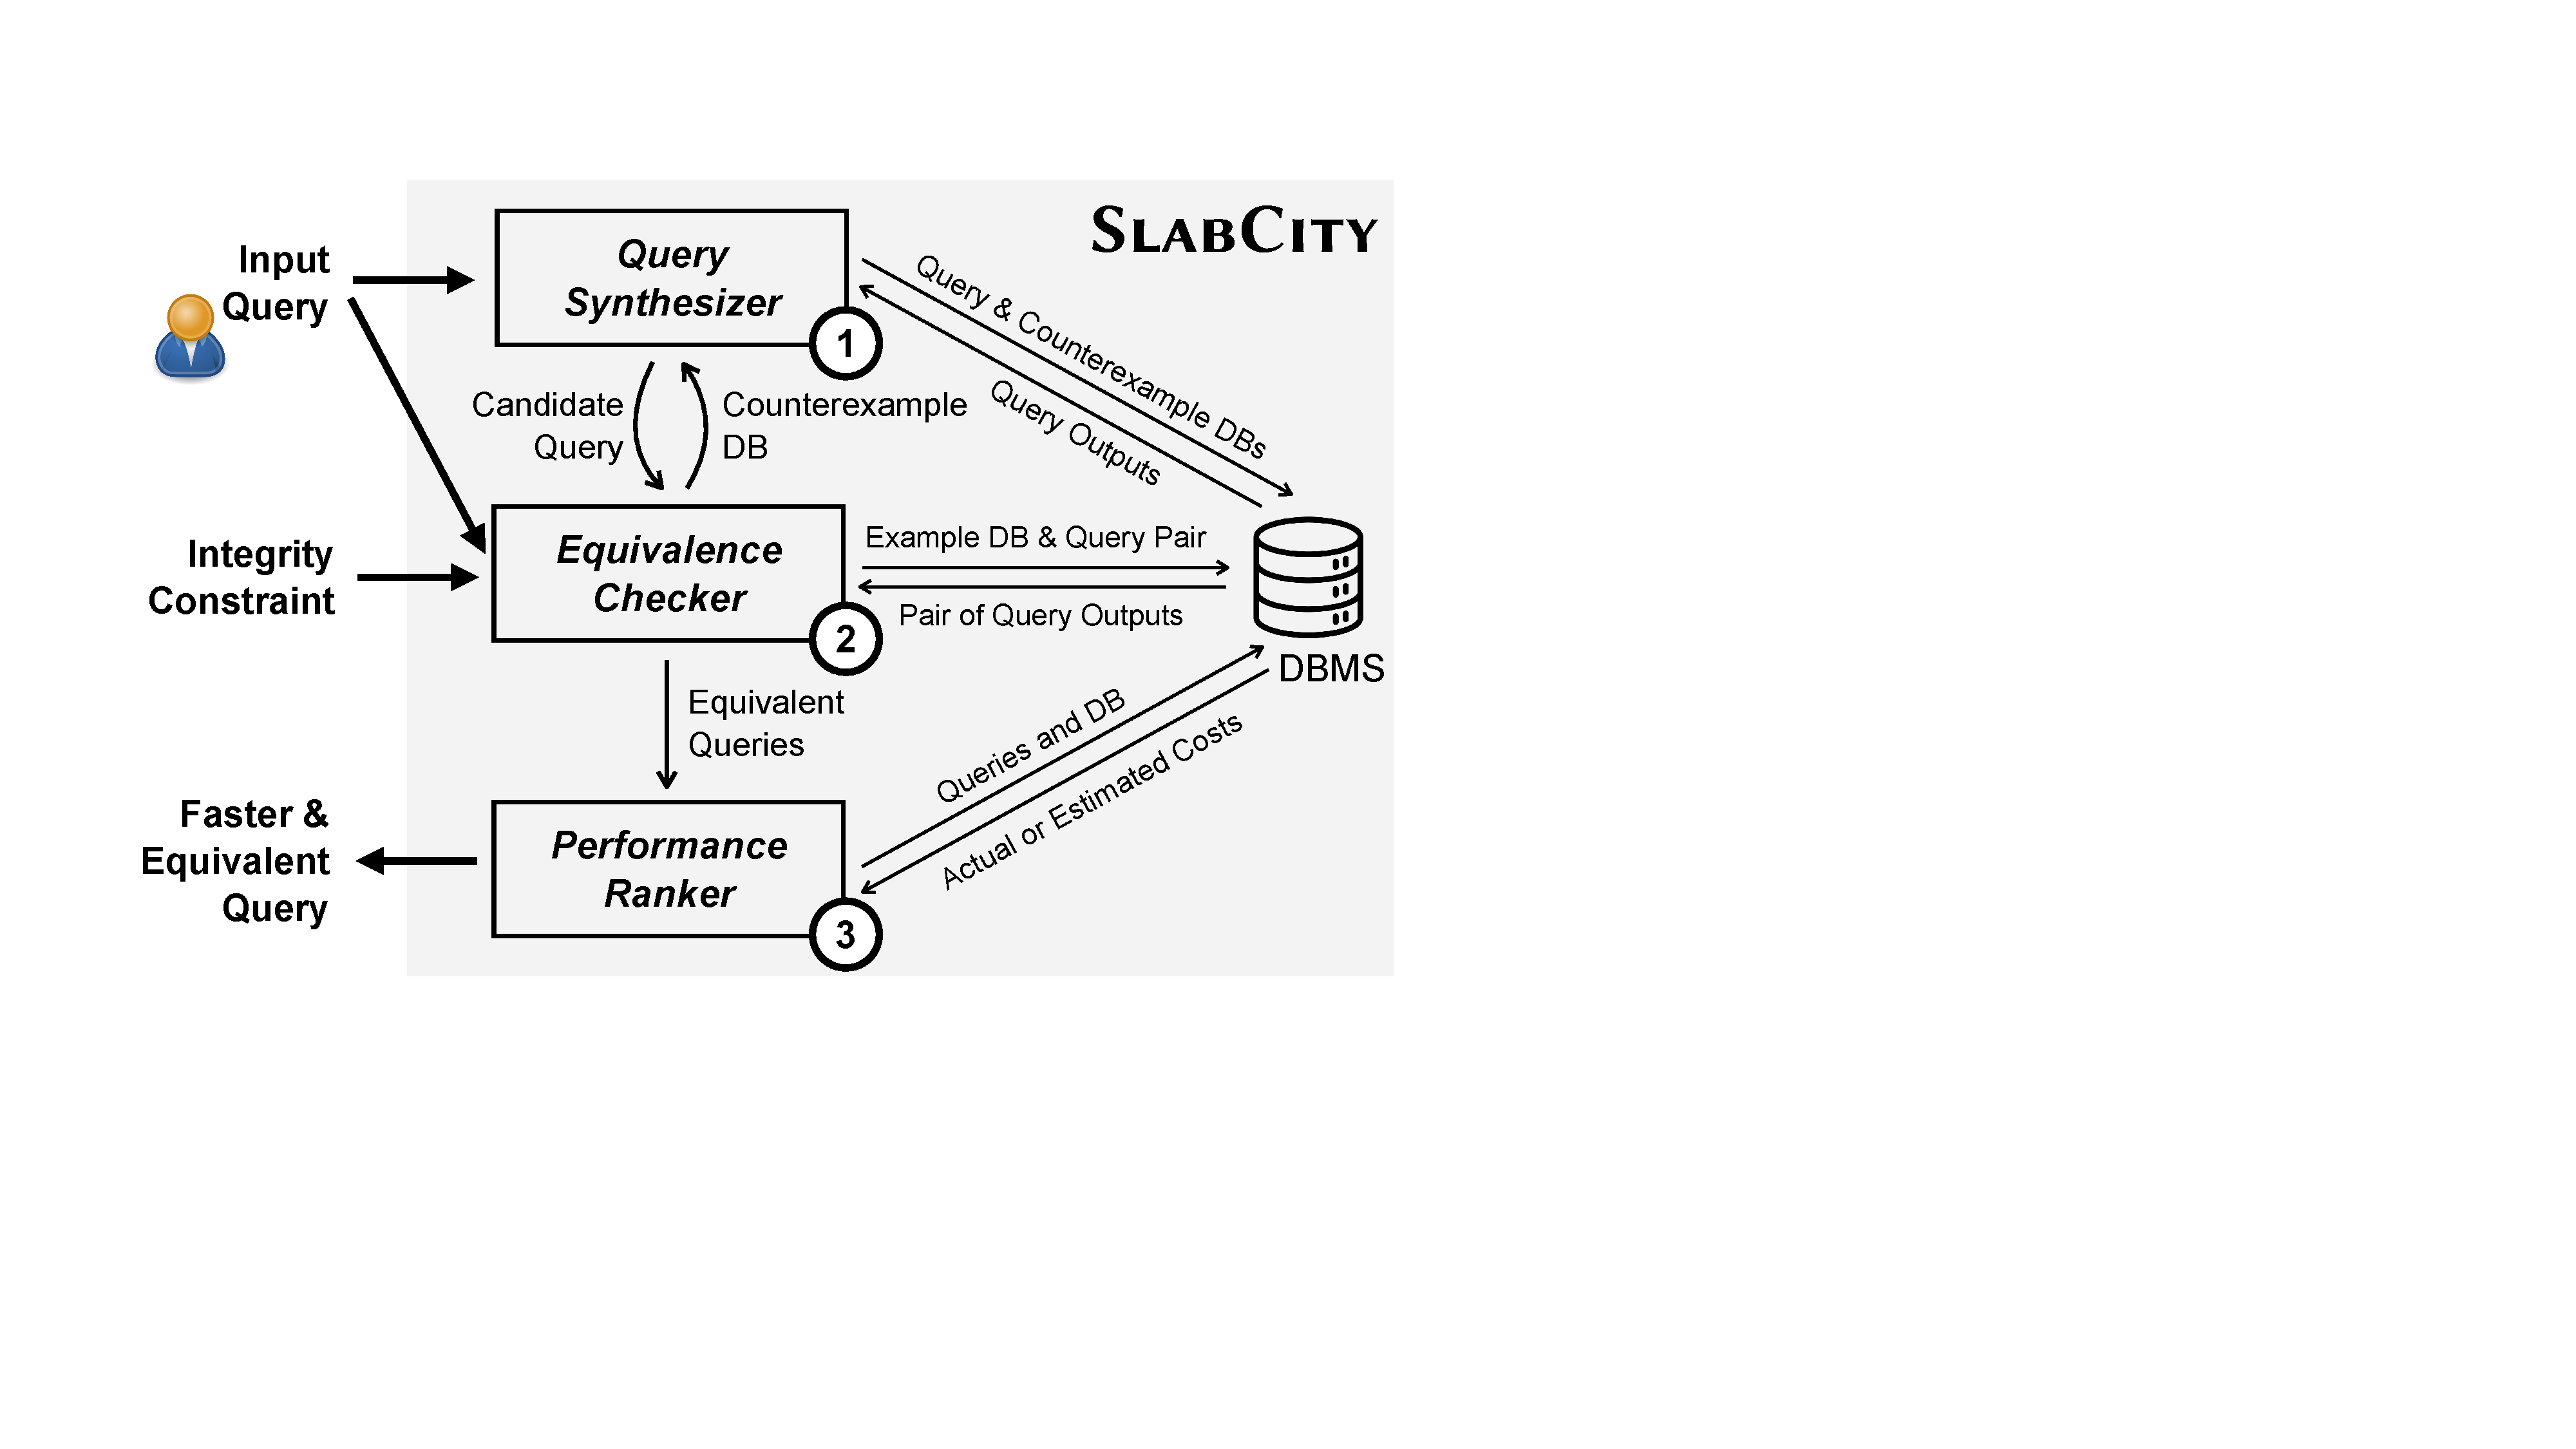
\includegraphics[width=0.8\linewidth]{chapters/slabcity/figs/workflow-clean.pdf}
\vspace{-5pt}
\caption{Schematic workflow of \slabcity.}
\vspace{-10pt}
\label{slab:fig:workflow}
\end{figure}

At the system level, \slabcity takes a query and the integrity
constraints of its schema and returns a semantically equivalent query
expected to run faster. \Cref{slab:fig:workflow} shows the
architecture, which instantiates the counterexample-guided inductive
synthesis (CEGIS) loop introduced in Chapter~2. A dataflow-guided
synthesizer proposes candidates that agree with the input query on all
counterexample databases collected so far. Each candidate then faces
the layered equivalence checker: a fast tester that hunts for a
distinguishing database, a bounded verifier that proves agreement on
all small inputs, and a full verifier that, when it succeeds within
its budget, establishes equivalence outright. A candidate refuted by
the tester or by the bounded verifier yields a new counterexample
database that sharpens the synthesizer's next proposals; a refutation
by the full verifier arrives as a verdict rather than a witness, and
simply discards the candidate. A candidate that survives is labeled
with the strongest guarantee it earned: fully verified, verified on
all bounded inputs, or, when the verifiers cannot reach a conclusion
within their budgets, tested. Surviving candidates are ranked by
measured or estimated latency, and the fastest is returned with its
label; a fully verified rewrite can be deployed as is, while the
weaker labels route the rewrite for human inspection.

\slabcity is aimed at workloads where a few seconds of one-time search
effort is negligible against the query's lifetime cost. That covers
queries written once and executed indefinitely, dashboards and the
query templates embedded in database-backed applications, and it
covers long-running analytical queries, where even a single execution
dwarfs a five-second rewriting budget. In both settings the rewriter
runs as a deployment-time step, after the query is written and before
it enters service. The supported language is an expressive subset of
SQL, including nested subqueries and arbitrary join structure; the
formal definition appears in \cref{slab:sec:problem}.

In summary, this chapter makes the following contributions:
\begin{itemize}[leftmargin=*]
\item
It introduces query dataflows: a semantic abstraction of SQL queries,
an algorithm for extracting the dataflows a query manifests, and the
observation that equivalent queries share dataflows, which converts an
undirected search space into a navigable one (a contribution of this
dissertation).
\item
It presents \slabcity, the first synthesis-based rewriter capable of
whole-query optimization with no rewrite rules, combining
dataflow-guided synthesis (due to Rui Dong, summarized here) with
layered equivalence checking (joint work).
\item
It contributes a benchmark of more than 1{,}000 real-life queries
curated from LeetCode, supporting research on query rewriting beyond
this chapter (joint work).
\item
It evaluates \slabcity against state-of-the-art rule-based and learned
rewriters across four workloads, showing that it optimizes 7 to 68\%
more queries and produces rewrites up to four orders of magnitude
faster (joint work).
\end{itemize}

The rest of the chapter proceeds as follows.
\Cref{slab:sec:motivating-example} illustrates, through queries drawn
from real workloads, the rewrites that rule-based systems miss and
this chapter's approach finds. \Cref{slab:sec:problem} defines the
query language and the rewriting problem precisely.
\Cref{slab:sec:dataflow} develops the dataflow abstraction, the
technical core of the chapter. \Cref{slab:sec:synthesis} summarizes
how the synthesis algorithm consumes dataflows to drive the search,
and \cref{slab:sec:eval} presents the evaluation. Related work,
including the two prior systems that apply synthesis to query
rewriting under rule-based or locality
restrictions~\cite{zhou2021sia,wang2022optimizing}, is discussed in
\cref{chap:related}.

\section{Motivating Examples}
\label{slab:sec:motivating-example}

In this section, we present a few examples to highlight the inherent limitations of rule-based 
query rewriting techniques and motivate the need for a synthesis-based whole-query optimization approach. 


All examples in this section are from two workloads: (1) real-life queries written by LeetCode users, 
%\footnote{The world's most popular online programming platform: https://leetcode.com/} users, 
and (2) benchmark queries from the Apache Calcite project~\cite{calcite}.
%\footnote{https://calcite.apache.org/}. 
We later present more comprehensive experiments on both workloads among others in Section~\ref{slab:sec:eval}. 
%but here we only use a handful of them as motivating examples.

\head{Example 1. Optimization with window functions} 
Consider LeetCode problem \#1308: a competition is held among teams of different genders. Given the table called \texttt{scores} with three columns \texttt{(gender,day,score)} where \texttt{(gender,day)} is the primary key, the goal is to find the running total score for each gender on each day. 
$\query_1$ in Table~\ref{slab:tab:Q1-Q2}  is the human-written solution for this problem (submitted by LeetCode participants) while 
$\query_2$ is \slabcity's automatically generated query after rewriting $\query_1$. 
$\query_2$ is more than 2000x faster than $\query_1$ on a database randomly populated with 1 million rows. 

\begin{table}[!t]
\footnotesize
\caption{$\query_1$ is human-written. $\query_2$ is generated by $\slabcity$.}
\vspace{-5pt}
\begin{tabular}{|c|c|}
\hline
 $\query_1$

 & 
 
 \makecell[l]{\sqlselectcolor \  \sqldistinctcolor s1.gender, s1.day, \sqlsumcolor(s2.score)\\
              \sqlfromcolor scores \sqlascolor s1 \sqljoincolor scores \sqlascolor s2 \\
              \hspace{2em} \sqloncolor s1.gender = s2.gender\\
              \sqlwherecolor s2.day <= s1.day \\
              $\sqlgroupbycolor$ s1.gender, s1.day
              }  
\\
\hline
$\query_2$
&
 \makecell[l]{ \sqlselectcolor gender, day, \\ \hspace{1em} \sqlsumcolor(score) \sqlovercolor (\sqlpartitionbycolor gender \sqlorderbycolor day) \\
 \sqlfromcolor scores}
  \\
 \hline
\end{tabular}
% \vspace{5pt}

\vspace{-5pt}
\label{slab:tab:Q1-Q2}
\end{table}



$\query_1$ is slow for two reasons. First, it uses a self-join to compute the running total, which generates a massive intermediate result. 
The same running total can be obtained using a window function as shown in $\query_2$. Second, the use of \sqldistinctcolor in $\query_1$ is redundant, since \texttt{(gender,day)} is the primary key. 

%\head{Limitations of rule-based techniques}

It is difficult to express any local rewrite rule to do this kind of optimization for $\query_1$ because nearly every part of the query would have to change. Moreover, anticipating these kinds of patterns in advance and writing a rule for each would be tedious (if not impossible). 
Even if one can create rules for a query like $\query_1$, many constraints would need to be met to ensure correctness, necessitating a potentially very complex pattern-matching. 
%and a very complex pattern matching would be needed. 
However, \slabcity's synthesis-based optimization can deal with such cases easily because, instead of doing constraint checking and pattern-matching, \slabcity~\emph{directly} searches the query language (as defined in Figure~\ref{slab:fig:querysyntax}),
allowing it to discover semantically equivalent and faster queries that may be quite different \emph{syntactically}. 
For these reasons, none of the state-of-the-art rule-based rewriters, such as {\learnedrewrite} (\LR)~\cite{LR} and {\wetune} (\WT)~\cite{wetune}, were able to optimize $\query_1$.\footnote{We explain how these state-of-the-art query rewriters work in more detail and report comprehensive experimental results in Section~\ref{slab:sec:eval}.}


%We will also use $(\query_1, \query_2)$ as a running example in Section~\ref{slab:sec:alg} to help illustrate details of our technique. 


\head{Example 2. Exploiting integrity constraints} 
The following is LeetCode problem \#1821.  
Given table \texttt{customers} with columns \texttt{(cid,year,revenue)} and \texttt{(cid,year)} as its primary key, the goal is to report  customers with positive revenue in  the year 2021. 
$\query_3$ from Table~\ref{slab:tab:Q3-Q4} is the human-written solution\footnote{While a database expert might be surprised why the user missed the integrity constraint and wrote such an inefficient query in the first place, situations like this are quite common in the industry for two reasons: (1) most queries are rewritten by users who are not SQL proficient, such as business users and financial analysts~\cite{slow-query-impact-5,slow-query-impact-7}
% ~\cite{Jie/Rui plz find a lot of links online to posts where ppl complain about poorly written SQL queries and cite them here} \xinyu{Jie: add cites here?} \jie{working on this}
, and (2) modern warehouses have hundreds of tables, and the knowledge of the schema and integrity constraints are thus scattered across different teams, especially in larger organizations~\cite{arora2011schema,stein2014enterprise}.
% ~\cite{Jie/Rui see if you can find some links supporting this. i know this is true anecdotally}. \xinyu{Jie/Rui: add cites?} \jie{working on this}
}  
for this task, while 
$\query'_4$ and $\query_4$ are $\slabcity$'s automatically generated queries for $\query_3$, which 
are  1.27x and 5.47x faster respectively (on a database with 1M rows).
$\slabcity$ can generate both $\query_4'$ and $\query_4$ but returns the latter due to its superior performance.

\begin{table}[!t]
\footnotesize 
\caption{$\query_3$ is human-written. $\query'_4$ and $\query_4$ are discovered by \slabcity ($\query_4$ is the final output as its faster than $\query'_4$).}
\vspace{-5pt}
\begin{tabular}{|c|c|}
\hline
 $\query_3$

 & 
 
 \makecell[l]{\sqlselectcolor cid\\
 \sqlfromcolor (\sqlselectcolor cid, \sqlsumcolor(revenue) \\ 
 \hspace{7.2em} \sqlovercolor (\sqlpartitionbycolor cid, year) \sqlascolor r \\
             \hspace{2.3em} \sqlfromcolor customers \  \sqlwherecolor year = 2021) \sqlascolor tmp \\
               \sqlwherecolor r > 0
              }  
\\

\hline

$\query_4'$

&

 \makecell[l]{ \sqlselectcolor cid \ \sqlfromcolor customers \ \\ \sqlwherecolor year = 2021 \\ 
                $\sqlgroupbycolor$ cid \  \sqlhavingcolor \sqlsumcolor(revenue) > 0}
 
 \\

 
\hline
$\query_4$
&
 \makecell[l]{
 \sqlselectcolor cid \ 
 \sqlfromcolor customers \\ 
 \sqlwherecolor year = 2021 \sqlandcolor revenue > 0
              }  
  \\
  
 \hline
\end{tabular}
\vspace{-8pt}

% \vspace{-20pt}
\label{slab:tab:Q3-Q4} 
\end{table}

%Capturing this kind of rewrite for rule-based techniques is inherently difficult as their ability to exploit integrity constraints is rather weak. For example, they are comfortable with checking if a single column is primary key so that a specific rule can be applied but they cannot infer if a single column (not primary key) is unique given a set of integrity constraints, which requires reasoning ability. As a result, syntactic pattern matching needs to be used more heavily to make up for their weak constraint checking, which is error-prone and still incomplete. In contrast, since \slabcity is not restricted to rules, as long as there is an optimal query in the search space, it will eventually find it.


$\query_3$ is slow because it uses an unnecessary window function with $\sqlpartitionbycolor$. $\query'_4$ achieves the same goal faster by replacing the window function with aggregation and $\sqlgroupbycolor$. This is because \texttt{(cid,year)} is the primary key --- once \texttt{year} is fixed, there is only a tuple for each unique value of \texttt{cid}. 
That is, partitioning by \texttt{(cid,year)} and grouping by \texttt{cid} when  \texttt{year=2021} leads to the same groups. 
Exploiting this integrity constraint further, 
\slabcity is able to find an even more optimized query $\query_4$.
This is because 
each \texttt{(cid,year)} will also determine a unique \texttt{revenue}, making the summation unnecessary.  
However, none of the state-of-the-art rule-based techniques could optimize or even rewrite $\query_3$ to anything. 
Capturing this kind of rewrite for rule-based techniques is nearly impossible, as they heavily rely on pattern-matching and their ability to exploit integrity constraints is largely limited to local changes (e.g., removing redundant grouping columns or redundant left joins).
In contrast, because \slabcity is  not restricted to rewrite rules fundamentally, as long as there is a better query in the query space, it will eventually find it. 



\head{Example 3. Eliminating redundant joins} 
Calcite comes with a rich set of test cases to check if its rewrite rules function properly.
$\query_5$ in Table~\ref{slab:tab:Q5-Q7} is one of those test cases (``testPushAggregateThroughOuterJoin14'') where 
Calcite rewrites $\query_5$ to  $\query_6$. Here, \texttt{emp} is a table with three columns \texttt{(empno,ename,mgr)} with \texttt{empno} as its primary key. 
$\query_5$ performs a full self-join of \texttt{emp} on the \texttt{mgr} column, grouped by the join key. This is 
essentially equivalent to using \sqldistinctcolor to return only distinct values. 
$\query_6$ is the optimized query using Calcite rules, which is 926x faster than $\query_5$ on a database with 4M rows. $\query_7$ is the query  automatically generated by \slabcity, which is 1833x faster than $\query_5$ on the same database. 


\begin{table}[!t]
\footnotesize
\caption{$\query_5$ is a test query from Calcite, 
$\query_6$ is the rewritten version of $\query_5$ using Calcite rules, and
$\query_7$ is \slabcity's output.}
\vspace{-8pt}
\begin{tabular}{|c|c|}
 \hline
 $\query_5$ 

 & 
 
 \makecell[l]{\sqlselectcolor e0.mgr \sqlascolor mgr0, e1.mgr \sqlascolor mgr1 \\
             \sqlfromcolor emp \sqlascolor e0 \sqlfulljoincolor emp \sqlascolor e1 \sqloncolor e0.mgr = e1.mgr\\
              $\sqlgroupbycolor$ e0.mgr, e1.mgr
              }  
\\

\hline

 $\query_6$ 

 & 
 
 \makecell[l]{\sqlselectcolor e0.mgr \sqlascolor mgr0, e1.mgr \sqlascolor mgr1 \\
             \sqlfromcolor (\sqlselectcolor mgr \sqlfromcolor emp $\sqlgroupbycolor$ mgr) \sqlascolor e0\\
            \hspace{1em} \sqlfulljoincolor (\sqlselectcolor mgr \sqlfromcolor emp $\sqlgroupbycolor$ mgr)  \sqlascolor e1 \\
            \hspace{1em} \sqloncolor e0.mgr = e1.mgr\\
              $\sqlgroupbycolor$ e0.mgr, e1.mgr
              }  
\\

\hline

 $\query_7$ 

&

 \makecell[l]{\sqlselectcolor mgr \sqlascolor mgr0, mgr \sqlascolor mgr1 \\
             \sqlfromcolor emp \\ $\sqlgroupbycolor$ mgr
              }  
\\
 \hline
\end{tabular}


\vs
\label{slab:tab:Q5-Q7} 
\vspace{5pt}
\end{table}

$\query_6$ is significantly faster than $\query_5$ because pushing $\sqlgroupbycolor$ before the self-join leads to  significantly smaller join operands and thus a more efficient execution; however, this is still not the best rewrite possible. Interestingly, self-join can be eliminated altogether in this case, leading to an even more significant speed-up, which is exactly what \slabcity does by rewriting $\query_5$ into $\query_7$. 
In fact, this is not limited to Calcite:
none of the state-of-the-art rule-based query rewriters found this opportunity,\footnote{Similar to Calcite, LearnedRewrite~\cite{LR} was only able to rewrite $\query_5$ into $\query_6$ but did not eliminate the self-join. WeTune was not able to rewrite $\query_5$ at all.} 
simply because they fail to capture the information that the joined columns may come from the same table and hence be identical --- a fact that could be exploited to eliminate redundancy. 
Similar to Examples 1 and 2, it is tedious, if not impossible, to create rewrite rules for this type of optimization.
In particular, identifying self-joins requires semantic information that the two joined operands are essentially the same relation. Even if one wrote a very specific rule for\\
\texttt{\sqlfromcolor T AS T1 \sqljoincolor T AS T2}\\
to find self-joins syntactically, they would still miss out on queries expressed as \\
\texttt{\sqlfromcolor T AS T1 \sqljoincolor (\sqlselectcolor * from T) AS T2} \\ 
In contrast, because of using query synthesis, $\query_7$ is naturally within \slabcity's search space and \slabcity can successfully find it as a query with minimal redundancy and best performance.




\begin{table}[!t]
\footnotesize
\caption{$\query_8$ is a test query from Calcite, 
$\query_9$ is the rewrite using Calcite rules, and
$\query_{10}$ is \slabcity's output.}
\vspace{-8pt}
\begin{tabular}{|c|c|}

 \hline
 $\query_8$

 & 
\makecell[l]{\sqlselectcolor ename, \sqlmincolor (empno) \sqlascolor e \sqlfromcolor (\\
             \hspace{1em} \sqlselectcolor * \sqlfromcolor emp \\
             \hspace{1em} \sqlunionallcolor\\
             \hspace{1em} \sqlselectcolor * \sqlfromcolor emp\\
              ) \sqlascolor t $\sqlgroupbycolor$ ename
              } 
 
  
\\

 \hline
 $\query_9$

 & 
\makecell[l]{\sqlselectcolor ename, \sqlmincolor (e) \sqlascolor e \sqlfromcolor (\\
             \hspace{1em} \sqlselectcolor ename, \sqlmincolor (empno) \sqlascolor e \sqlfromcolor emp $\sqlgroupbycolor$ ename\\
             \hspace{1em} \sqlunionallcolor\\
             \hspace{1em} \sqlselectcolor ename, \sqlmincolor (empno) \sqlascolor e \sqlfromcolor emp $\sqlgroupbycolor$ ename\\
              ) \sqlascolor t $\sqlgroupbycolor$ ename
              } 
 
  
\\

\hline

 $\query_{10}$

&
\makecell[l]{\sqlselectcolor ename, \sqlmincolor (e) \sqlascolor e \\ \sqlfromcolor (\sqlselectcolor ename, \sqlmincolor (empno) \sqlascolor e
             \\ 
             \hspace{2.4em} \sqlfromcolor emp 
             \\ \hspace{2.4em} $\sqlgroupbycolor$ ename) \sqlascolor t
             \\
             $\sqlgroupbycolor$ ename
              } 
  
 
 \\
 \hline
\end{tabular}
\vspace{-15pt}


\label{slab:tab:Q8-Q10} 
\end{table}




\head{Example 4. Optimizating set operations}
$\query_8$ in Table~\ref{slab:tab:Q8-Q10} is yet another test case (``testPushMinThroughUnion'') from Calcite, 
which is rewritten to $\query_9$ using Calcite rules, slightly improving its latency ($\pm$2\%) by pushing $\sqlgroupbycolor$ past $\sqlunionallcolor$. 
On the other hand, \slabcity rewrites $\query_9$ to $\query_{10}$, which is 1.7x faster. 


Similar to Example 3, state-of-the-art rule-based rewriters fail to exploit the fact that both sides of $\sqlunionallcolor$ are identical, and thus fail to eliminate the redundant computation. 
In fact, neither \learnedrewrite nor \wetune were able to optimize $\query_8$ (the former could rewrite it to $\query_9$ whereas the latter was not even able to rewrite it to anything at all).
%\barzan{jie, plz go through the whole paper and see how we refer to LR and WT, do we use these acronyms everywhere? If so, let's define them the first timr we reference them and use the same everywehre consistently} \jie{We first use it in example 1 (page 3). I am not sure if I "define" it properly there. Please check}
Again, because $\slabcity$ uses query synthesis, it is able to find $\query_{10}$ which is both equivalent and faster.


\head{Discussion}
In our evaluation, we have come across many other interesting examples where state-of-the-art query rewriting techniques were not able to optimize the input query or even rewrite it at all, while \slabcity could (see Section~\ref{slab:sec:q1-coverage}).
Even when they were able to optimize the query, \slabcity's output oftentimes was significantly faster (see Section~\ref{slab:sec:q2-reduction}). 
Note that in this paper, we differentiate two terms \emph{optimize} vs. \emph{rewrite}: the former means the technique can rewrite the input query to an output query that is faster, whereas the latter means the technique can rewrite to some query which may or may not be faster. In other words, optimizing is harder than rewriting. 
Our intention of sharing these motivating examples in Section~\ref{slab:sec:motivating-example} is to demonstrate why it is inherently difficult and error-prone to create enough rules that can handle complex and unseen situations. In contrast, a synthesis-based approach does not need a supply of hard-coded rules and can discover optimization opportunities by searching the SQL language \emph{directly}.

\begin{comment}
\barzan{Xinyu, this is why i think its better to not use rewrite and optimize interchangeably. if you agree, plz add the clarification the first time it occurs that optimize means rewriting into a faster query.}
Even when they were able to optimize the query, \slabcity's output was significantly faster (see Section~\ref{slab:sec:??}). 
Interestingly, we even identified several examples where these techniques produced an incorrect query (see \barzan{appendix or tech report or supp material? if this stmt is not true then eliminate this sentence} \jie{this stmt is true and I think we can add some examples as the proof})
Our intention of sharing these motivating examples in this section to show the reader why it is inherently difficult, error-prone, and extremely difficult \jie{(inherently difficult, extremely difficult) repeat?} to create enough rules that can handle 
complex and unseen situations. In contrast, a synthesis approach does not need a supply of hard-coded rules and can discover optimization opportunities by searching the languauge space directly.
\barzan{Xinyu, reword or add this para if you want}
\end{comment}


\section{Problem Setup}
\label{slab:sec:problem}

This section fixes the search space and the goal: the query language
\toolname operates over, the integrity constraints it can exploit, and
the problem it solves.

%\subsection{Query Space}
%\label{slab:sec:querylanguage}

\head{Query space}
The language, defined in Figure~\ref{slab:fig:querysyntax}, is an
expressive subset of SQL covering arbitrary nesting and join
structure.
%\slabcity currently supports a wide subset of SQL queries, including arbitrary nesting and join patterns. See Figure~\ref{slab:fig:querysyntax} for the formal language currently supported by \slabcity.



%\subsection{Integrity Constraints}
%\label{slab:sec:integrityconstraints}

\head{Integrity constraints}
Constraints both shrink the space of databases against which
equivalence must hold and, as Example~2 of
\cref{slab:sec:motivating-example} illustrated, create rewrite
opportunities. \slabcity supports the following kinds:
\begin{itemize}[leftmargin=*]
\item 
Primary and foreign keys. 
\item 
Comparisons within a row --- e.g.,  $\texttt{T.StartTime} < \texttt{T.EndTime}$. 
\item 
Implication constraints within a row. For example, $\texttt{T.EmailType} \neq \emph{spam} \rightarrow \texttt{T.action} = \texttt{NULL}$. 
%means if column \texttt{EmailType} is not \emph{spam} then column \texttt{action} is \texttt{NULL}. 
\item 
Whether or not a column can be \texttt{NULL}. 
\item 
Range constraints (for columns of integer or numeric types).
\item 
Enum types (e.g., column \texttt{Device} can draw from \{ \emph{S8}, \emph{iPhone} \}).
\end{itemize}

\begin{comment}
\begin{enumerate}
    \item primary keys
    \item foreign keys
\item comparative constraints within a row, e.g. \texttt{T.StartTime < T.EndTime} 
    \item implication constraints within the same row, e.g. \texttt{T.EmailType != "spam" -> T.action = NULL} means if the value of column \texttt{EmailType} is not \texttt{"spam"}, then the value of column \texttt{action} is \texttt{NULL}
        \item whether or not a column can be \texttt{NULL}
    \item range constraints (for int or numeric type columns)
    \item enum types, e.g. column \texttt{Device} can only take values from the set \texttt{\{"S8", "iPhone"\}}
    %\item \tofix{special constraints within a column, including 1) values of a column are incremental, 2) values of a column are consecutive.} \barzan{this one is a bit strange, what is the actual name of this kind of constraint in Oracle? auto increment is a feature not an IC afaik}     \xinyu{I think this one is very rare in the benchmarks. we do not have to include this one in the list.}
\end{enumerate}
\end{comment}


\head{Problem statement}
With the language and constraints in place, the problem is the
following.
%\subsection{Query Optimization Problem Statement}
%\label{slab:sec:problemstatement}

\begin{definition}
Given a query $\inputquery$ and an integrity constraint $\dataconstraint$, find a query $\query$ from our query language, such that the following two conditions hold: 
\begin{enumerate}[leftmargin=*]
\item 
$\query$ is semantically equivalent to $\inputquery$ with respect to $\dataconstraint$. 
That is, $\query$ and $\inputquery$ produce the same output on any database $\inputdb$ that meets the integrity constraint $\integrityconstraint$. 
\item 
$\query$ runs faster than $\inputquery$. Here, query performance is measured using \texttt{EXPLAIN} or the actual execution of the query.
\end{enumerate}
\label{slab:def:problem}
\end{definition}

Two aspects of the definition deserve a remark. Equivalence is
relative to the constraints, which is what licenses rewrites like
$\query_4$ in \cref{slab:sec:motivating-example}: they would be wrong
on arbitrary databases and are right on the databases that can
actually occur. And the definition asks for a faster query, not just
an equivalent one, which is why the system must surface multiple
equivalent candidates and rank them (\cref{slab:sec:perfranking}),
rather than stop at the first equivalence it can prove.



\begin{figure}[!t]
\footnotesize
\centering
\[
\arraycolsep=1.5pt\def\arraystretch{1.1}
\begin{array}{rrll}

\emph{Query} & 
\query & 
\grammareq & 
\emph{an input table} \\ 
& & \ \ \ | &  
\sqlselect \sqlspace \targetlist \sqlspace \sqlfrom \sqlspace \query \sqlspace \sqlwhere \sqlspace \sqlpredicate \\ 
& & \ \ \ | &  
\sqlselect \sqlspace \targetlist \sqlspace \sqlfrom \sqlspace \query \sqlspace \sqlgroupby \sqlspace \cols \sqlspace \sqlhaving \sqlspace \sqlpredicate \\ 
& & \ \ \ | &  
\sqlselect \sqlspace \targetlist \sqlspace \sqlfrom \sqlspace \query \sqlspace \sqlorderby \sqlspace \cols  \\ 
& & \ \ \ | &  
\query \sqlspace \sqlinnerjoin \sqlspace \query \sqlspace \sqlon \sqlspace \sqlpredicate \\ 
& & \ \ \ | &  
\query \sqlspace \sqlleftjoin \sqlspace \query \sqlspace \sqlon \sqlspace \sqlpredicate 
%& & \ \ \ | &  
%\query \sqlspace \sqlrightjoin \sqlspace \query \sqlspace \sqlon \sqlspace \sqlpredicate 
\\[2pt]

\emph{Target List} & 
\targetlist & 
\grammareq & 
[ \target \sqlspace \sqlas \sqlspace \colalias, \mydots, \target \sqlspace \sqlas \sqlspace \colalias ]
\\
& & \ \ \ | &  
\sqldistinct \sqlspace [ \target \sqlspace \sqlas \sqlspace \colalias, \mydots, \target \sqlspace \sqlas \sqlspace \colalias ] 
%\rui{add DISTINCT?}
\\[2pt]

\emph{Target} & 
\target & 
\grammareq & 
\col \ | \ \agg(\col) \ | \ \agg( \sqldistinct \sqlspace \col) 
%\rui{add DISTINCT?} 
\\
& & \ \ \ | &  
\agg(\col) \sqlspace \sqlover( \sqlpartitionby \sqlspace \cols \sqlspace \sqlorderby \sqlspace \cols )
\\ 
& & \ \ \ | &  
\windowfunc \sqlspace \sqlover( \sqlpartitionby \sqlspace \cols \sqlspace \sqlorderby \sqlspace \cols )
\\[2pt] 

\emph{Column List} & 
\cols & 
\grammareq & 
[\col, \mydots, \col]
\\[2pt]

\emph{Column} & 
\col & 
\grammareq & 
\colalias \ | \ \emph{a column from an input table} 
\\[2pt]

\emph{Condition} & 
\sqlpredicate & 
\grammareq & 
\sqlexpr \ \emph{op} \ \sqlexpr \ | \ \sqlpredicate \land \sqlpredicate \ | \ \sqlpredicate \lor \sqlpredicate 
\\[2pt] 

\emph{Expression} & 
\sqlexpr & 
\grammareq & 
\col \ | \ \agg(\col) \ | \ \agg(\sqldistinct \sqlspace \col) \ | \ \emph{const}
\\[2pt] 

\emph{Agg. Func.} & 
\agg & 
\grammareq & 
\sqlmax \ | \ \sqlmin \ | \ \sqlavg \ | \ \sqlsum \ | \ \sqlcount 
\\[2pt] 

\emph{Window Func.} & 
\windowfunc & 
\grammareq & 
\sqldenserank \ | \ \sqlrank 
\\[2pt] 

\end{array}
\]
\vspace{-15pt}
\caption{Syntax of our query language.}
\label{slab:fig:querysyntax}
\vspace{-20pt}
\end{figure}



\section{Synthesis-Aided Query Optimization}
\label{slab:sec:alg}


\revisioncancut{Section~\ref{slab:sec:toplevelalg} first presents a high-level overview of our synthesis-aided query optimization algorithm. 
Subsequent sections present the technical details of each component. 
We define dataflows for SQL queries --- which is one of our key contributions --- and use that to develop a monotonic scoring in Section~\ref{slab:sec:scorefunction}.
Section~\ref{slab:sec:prioritizingsearch} presents our query search algorithm. 
Finally, we describe how we check for equivalence and rank queries in  Sections~\ref{slab:sec:checkingequiv} and~\ref{slab:sec:perfranking}, respectively.}

 
\newcounter{mycounter}


\subsection{Top-Level Algorithm}
\label{slab:sec:toplevelalg}
Our top-level algorithm is shown in Algorithm~\ref{slab:alg:toplevelalg}. It accepts as input a query $\inputquery$ and an integrity constraint $\integrityconstraint$, and returns an output query $\query$ that is semantically equivalent to and faster than $\inputquery$. 
%In other words, if $\query$ passes our equivalence checker (line~\ref{slab:alg:toplevelalg:checkequiv}) and is ranked as faster than $\inputquery$ (line~\ref{slab:alg:toplevelalg:checkfaster}), then we return $\query$ at line~\ref{slab:alg:toplevelalg:returnquery}\footnote{For simplicity of our notation, here we only return the fastest query but one can also return the entire ranked list of rewritten queries to the user.}.
$\query$ is $\bot$ if it does not find one such query within the given time limit. 




Let us explain Algorithm~\ref{slab:alg:toplevelalg} in more detail. At a high-level, our algorithm is a \emph{new instantiation} of the counterexample-guided inductive synthesis (CEGIS) paradigm~\cite{solar2008program} --- which has found great success in the programming languages community --- for our query optimization problem. 
Our approach consists of (a) an inductive synthesizer (i.e., our query synthesizer) that aims to find a query $\query$ which satisfies a set $\counterexamples$ of \emph{counterexamples} and (b) a query checker (i.e., our equivalence checker) which checks whether or not $\query$ is equivalent to $\inputquery$ and generates a counterexample $\counterexample$ if not. 
One key advantage of using CEGIS is to enable efficient checking: checking a candidate query against $\counterexamples$ (line~\ref{slab:alg:toplevelalg:satisfycounterexample}) is typically significantly cheaper than calling an equivalence checker (line~\ref{slab:alg:toplevelalg:checkequiv}, e.g., \spes~\cite{zhou2022spes}). In other words, verification is used parsimoniously only when necessary. 
In our context, a counterexample $\counterexample$ is an input DB together with the desired output table returned by $\inputquery$. 




{In addition to using counterexamples, \toolname also uses a novel $\scorefunction$ function that defines dataflows for queries in order to guide the query synthesis process. 
While we defer the formal definition of $\scorefunction$ to Section~\ref{slab:sec:scorefunction}, from a high-level, it assigns a non-positive integer score\footnote{While \emph{non-positive} scores may seem counter-intuitive, they can be viewed as the negation of the cost, i.e., the higher the score, the lower the cost.} to each query $\query$ such that,  
$\query$ with a higher score is more likely to be an optimized query (i.e., semantically equivalent to and faster than $\inputquery$) and vice versa. 
Initially, $\counterexamples$ has no counterexamples and $\queryset$ is a empty set that stores equivalent queries (line~\ref{slab:alg:toplevelalg:init}). 
Then, we enter a CEGIS loop (lines~\ref{slab:alg:toplevelalg:whilebegin}--\ref{slab:alg:toplevelalg:whileend}). At line~\ref{slab:alg:toplevelalg:forloop}, it \emph{lazily} enumerates all queries in non-ascending order of their scores. In other words, $\toolname$ prioritizes the search for candidate queries $\query$ that are likely to optimize $\inputquery$ (i.e., with a higher score). 
Line~\ref{slab:alg:toplevelalg:satisfycounterexample} checks if $\query$ meets $\counterexamples$: if not, it continues to the next candidate. 
If $\query$ passes $\counterexamples$, we invoke the equivalence checker (line~\ref{slab:alg:toplevelalg:checkequiv}) to see if $\query$ is equivalent --- it returns a new counterexample $\counterexample$ if not equivalent, or returns $\emph{null}$ otherwise. 
For the latter case, line~\ref{slab:alg:toplevelalg:nocounterexample} adds $\query$ to $\queryset$; for the former, line~\ref{slab:alg:toplevelalg:addcounterexample} adds  $\counterexample$ to $\counterexamples$.
Upon termination, we rank queries in $\queryset$ (line~\ref{slab:alg:toplevelalg:checkfaster}) and return a ``best'' query that we believe can \emph{optimize} $\inputquery$.}



\begin{figure}[!t]
\vspace{-5pt}
\footnotesize
\centering

\begin{algorithm}[H]
\begin{algorithmic}[1]

\myprocedure{Optimize}{$\inputquery, \integrityconstraint$}

\Statex\Input{An input query $\inputquery$ and an integrity constraint $\integrityconstraint$.}


\Statex\Output{An equivalent and faster output query $\query$.}

\vspace{2pt}

\State $\counterexamples \assign \emptyset$; \  $\queryset \assign \emptyset$; 
\label{slab:alg:toplevelalg:init}



\While{not timed out}
\label{slab:alg:toplevelalg:whilebegin} 



\ForAll{$\query \in \textsc{LazyEnumerate}(\inputquery)$} \label{slab:alg:toplevelalg:forloop}
\Comment{{{\scriptsize \Circled{1}}} Query synthesizer.}


\State \textbf{if} $\query$ doesn't pass  $\counterexamples$ \textbf{then} \textbf{continue}; \label{slab:alg:toplevelalg:satisfycounterexample}
\Comment{Check against counterexs.}


\State $\counterexample \assign \textsc{CheckEquivalence}(\query, \inputquery, \integrityconstraint)$;\label{slab:alg:toplevelalg:checkequiv}
\Comment{{{\scriptsize \Circled{2}}} Equivalence checker.}

\vspace{1pt}

\If{$\counterexample = \emph{null}$} 
$\queryset.\emph{add}(\query)$
\label{slab:alg:toplevelalg:nocounterexample}
\Comment{$\emph{null}$ means $\query$ is equivalent to $\inputquery$.}

\Else \ $\counterexamples.\emph{add}( \counterexample )$;
\Comment{Otherwise, $\counterexample$ is a new counterexample.}
\label{slab:alg:toplevelalg:addcounterexample}

\EndIf

\EndFor


\EndWhile
\label{slab:alg:toplevelalg:whileend}

\vspace{-1pt}
\State $\query \assign \textsc{RankPerformance}(\queryset, \inputquery)$;
\label{slab:alg:toplevelalg:checkfaster}
\Comment{{{\scriptsize \Circled{3}}} Performance Ranker.}

\State \Return $\query$;
\label{slab:alg:toplevelalg:returnquery}

\caption{{Top-level algorithm of \toolname.}}
\label{slab:alg:toplevelalg}
\end{algorithmic}
\end{algorithm}
\vspace{-10pt}
\end{figure}





\begin{comment}
    
\begin{figure}[!t]
\small 
\centering

\begin{algorithm}[H]
\begin{algorithmic}[1]

\myprocedure{Optimize}{$\inputquery, \integrityconstraint$}

\Statex\Input{An input query $\inputquery$ and an integrity constraint $\integrityconstraint$.}


\Statex\Output{An equivalent and faster output query $\query$.}

\vspace{2pt}

\State $\counterexamples \assign \emptyset$; \  $\cost = 0; \ \queryset \assign \emptyset$; 
\label{slab:alg:toplevelalg:init}



\While{not timed out}
\label{slab:alg:toplevelalg:whilenottimeout} 



\ForAll{$\query \in \textsc{LazyEnumerate}(\cost)$} \label{slab:alg:toplevelalg:forloop}
\Comment{{{\scriptsize \Circled{1}}} Query synthesizer.}


\State \textbf{if} $\query$ doesn't pass  $\counterexamples$ \textbf{then} \textbf{continue}; \label{slab:alg:toplevelalg:satisfycounterexample}
\Comment{Check against counterexs.}


\State $\counterexample \assign \textsc{CheckEquivalence}(\query, \inputquery, \integrityconstraint)$;\label{slab:alg:toplevelalg:checkequiv}
\Comment{{{\scriptsize \Circled{2}}} Equivalence checker.}

\vspace{1pt}

\If{$\counterexample = \emph{null}$} 
$\queryset.\emph{add}(\query)$
\label{slab:alg:toplevelalg:nocounterexample}
\Comment{$\emph{null}$ means $\query$ is equivalent to $\inputquery$.}

\Else \ $\counterexamples.\emph{add}( \counterexample )$;
\Comment{Otherwise, $\counterexample$ is a new counterexample.}
\label{slab:alg:toplevelalg:addcounterexample}

\EndIf

\EndFor

\vspace{-2pt}
\State $\cost \assign \cost - 1$;
\label{slab:alg:toplevelalg:decreasescore} 

\EndWhile

\vspace{-1pt}
\State $\query \assign \textsc{RankPerformance}(\queryset, \inputquery)$;
\label{slab:alg:toplevelalg:checkfaster}
\Comment{{{\scriptsize \Circled{3}}} Performance Ranker.}

\State \Return $\query$;
\label{slab:alg:toplevelalg:returnquery}

\caption{Top-level algorithm of \toolname.}
\label{slab:alg:toplevelalg}
\end{algorithmic}
\end{algorithm}
\vspace{-20pt}
\end{figure}

\end{comment}



\begin{example}
Suppose $\inputquery$ is query $\query_1$ from Table~\ref{slab:tab:Q1-Q2}. 
Our CEGIS-based algorithm will begin with query candidates with score 0: $\query'$ below is one such query. 
$\query'$ is obviously not equivalent to $\inputquery$, and our equivalence checker gives a counterexample $\counterexample$ below. Note that $\counterexample$ consists of an input DB $\inputdb$ and the output that $\inputquery$ returns on $\inputdb$. 
A query eventually returned by our tool will pass this counterexample. 



\begin{table}[H]
\footnotesize
\caption*{A counterexample $\counterexample$ consists of an input database $\inputdb$ (left) and an output table of $\inputquery$ on $\inputdb$.}
\vspace{-7pt}
\hspace*{-5pt}
\begin{tabular}{cc}
\makecell[l]{ $\query': $ \ \sqlselectcolor gender, day, \\  
\hspace{42pt} \sqlsumcolor(score) 
  \\ \hspace{2em} \sqlfromcolor scores
  \\ \hspace{2em} $\sqlgroupbycolor$ gender, day}
  &
\makecell[l]{ $\query\doubleprime: $ \sqlselectcolor gender, day, \\
\hspace{5.3em} \sqlsumcolor(score) \\  \hspace{5.3em} \sqlovercolor ($\sqlpartitionbycolor$ gender \\ \hspace{7.9em} $\sqlorderbycolor$ day)\\
 \hspace{2em}  \  \sqlfromcolor scores \\ \hspace{2em} \  $\sqlgroupbycolor$ gender, day}
\end{tabular}
\vspace{-12pt}
\end{table}



\begin{table}[H]
\footnotesize
\begin{tabular}{cc}
\begin{subtable}{.4\linewidth}
\begin{tabular}{|c|c|c|}
 \hline
        gender & day & score \\
        \hline
        a & 1 & 1 \\
        a & 2 & 2 \\
        \hline
\end{tabular}
\end{subtable}
&
\begin{subtable}{.4\linewidth}
\begin{tabular}{|c|c|c|}
 \hline
        gender & day & score \\
        \hline
        a & 1 & 1 \\
        a & 2 & 3 \\
        \hline
\end{tabular}
\end{subtable}
\end{tabular}
%\caption{counterexample $\counterexample$}

\vspace{-5pt}
\label{slab:tab:alg:counterexample}
\end{table}



On the other hand, the query $\query\doubleprime$ next to $\query$ above is equivalent to $\inputquery$. However, $\query\doubleprime$ is determined to be slower than $\query_2$ from Table~\ref{slab:tab:Q1-Q2} by our performance ranker. 
$\toolname$ was able to find both $\query_2$ and $\query\doubleprime$ which are added to $\queryset$; however, \toolname returns $\query_2$ in the end, since it is ranked the highest. 


\label{slab:ex:cegis}
\end{example}


\subsection{Dataflow-Based Query Score Function}
\label{slab:sec:scorefunction}

As we can see, a key challenge underlying the success of Algorithm~\ref{slab:alg:toplevelalg} is how to design a good score function as well as how to develop an algorithm that can effectively use the score function to prioritize the search. 
This section first addresses the score function design. 


\head{Key idea: scoring queries based on dataflows}
Recall that we use a score function to quantitatively rank queries in terms of their likelihood of optimizing a user-provided input query $\inputquery$. That is, given $\inputquery$ and $\query$, a desired score function should assign $\query$ with a higher score if $\query$ is indeed semantically equivalent to and faster than $\inputquery$. At the same time, it should minimize false positives: that is, it should not assign high scores to too many inequivalent queries. 


To design such a score function, our key insight is that, a query $\query$ that indeed optimizes $\inputquery$ typically exhibits \emph{dataflows} that are also manifested in $\inputquery$. 
For example, if $\query$ filters an aggregated column (e.g., using $\sqlhaving \sqlspace \sqlsum$), the same computations (e.g., calculating $\sqlsum$) likely would also show up in $\inputquery$, although the computations might be organized \emph{syntactically differently} (e.g., first calculating $\sqlsum$ in $\sqlselect$ and then using $\sqlwhere$ to filter, which is slower). 
In other words, our dataflow-based score function is designed to favor queries $\query$ that involve dataflows from $\inputquery$ --- the rationale is that, since $\inputquery$ is functionally correct, its underlying computations are likely sufficient for generating an optimized query.


However, we do not require $\query$ to use up all dataflows from $\inputquery$. In other words, $\inputquery$ may exhibit redundant dataflows that are not necessary for computing the same result and thus can be optimized away. For example, if $\inputquery$ involves a redundant $\sqljoin$, an optimized query $\query$ may contain only dataflows from one branch of the $\sqljoin$. 


Finally, if a query $\query'$ contains dataflows that are not exhibited in $\inputquery$, oftentimes $\query'$ is not equivalent and hence we can assign it with a lower score. For example, suppose $\inputquery$ calculates $\sqlsum$ over a column. It is less likely that a query $\query'$ can accomplish the same goal with only $\sqlavg$. Similarly, if $\inputquery$ and $\query'$ both perform filtering but on two different columns that are unrelated, it is more plausible to believe they are not semantically equivalent. 
%However, special care needs to be taken for ``alternative dataflows'' --- that is, two syntactically different dataflows may share the same underlying logic. 
%For instance, $\sqlpartitionby$ and $\sqlgroupby$, while syntactically different, can both be used for grouping. 



\barzanrev{Note that, 
since our score is calculated based on semantic information (i.e., dataflows) instead of syntactic features, a syntactically simpler query (e.g., one with fewer lines) may receive a lower score than a more complex query. 
In other words, our algorithm first prioritizes generating queries with higher scores, and 
then prioritizes syntactically smaller queries when their scores are the same (see Section~\ref{slab:sec:prioritizingsearch}). This is an advantage since it will allow us to uncover non-trivial rewrites sooner if they are more promising.} 


\head{Dataflows}
Our observations suggest a score function design that takes two queries (i.e., $\inputquery$ to be optimized and $\query$ to be scored), extracts dataflows for each, and calculates the score based on these dataflows. 
In what follows, we first formalize the notion of dataflow.
Then, we present the dataflow extraction algorithm. 

\begin{definition}[Dataflow]
A dataflow $\dataflowchain$ (defined in Figure~\ref{slab:fig:dataflowlanguage}) for a given query $\query$ is a sequence of SQL operations that are performed during $\query$'s execution on one or more input tables or their columns.
\end{definition}


Let us explain our dataflow language more formally (see Figure~\ref{slab:fig:dataflowlanguage}).
In the base cases, a dataflow $\dataflowchain$ is either an input table $\dbtable$ or a column from an input table. 
%it must not be a column alias created for an intermediate table. 
%The reason is to make dataflows independent on specific intermediate results of a query. 
In the recursive cases, $\dataflowchain$ captures operations performed on top of such base dataflows. 
For example, $\agg(\dataflowchain, \mydots, \dataflowchain)$ describes the application of an aggregate function over dataflows for argument columns. 
$[\dataflowchain, \mydots, \dataflowchain]$ is the composition of columns to form a table (e.g., via $\sqlselect$). 
Expressions, such as $=$ and $\leq$, involves comparison logics, which is what $\emph{op}(\dataflowchain, \dataflowchain)$ is designed for. The language also includes boolean combinations of dataflows in order to represent dataflows from the filtering conditions in a query.
Finally, we capture other SQL operations, such as $\sqlpartitionby$, $\sqlorderby$, $\sqlgroupby$, etc.
%Note that we do not include all SQL operators (e.g., $\sqlselect$) since $\sqlselect$ is already implicitly taken into account by $[\dataflowchain, \mydots, \dataflowchain]$. 

\begin{example}
In this example, we show some sample dataflows for $\inputquery$ from Example~\ref{slab:ex:cegis}:
$$
\small
 \left \{
\text{\texttt{scores.score}, $\texttt{scores.day} \leq \texttt{scores.day}$, \sqlsumcolor(\texttt{scores.score}), $\dotsb$ }
\right \}
$$
We have \texttt{scores.score} because $\query_{\emph{in}}$ uses data from \texttt{score} column in \texttt{scores} table. 
We have \sqlsumcolor(\texttt{scores.score}), since $\query_{\emph{in}}$ performs summation on this column. 
Similarly, $\texttt{scores.day} \leq \texttt{scores.day}$ because an intermediate step of $\query_{\emph{in}}$ does a comparison between these two columns. 
%As we can see, $\query_{\emph{in}}$'s dataflows capture all operations in $\query_{\emph{in}}$.

\begin{comment}
\begin{table}[H]
\small
\begin{tabular}{|c|c|}
 \hline
 $\dataflowset_{\emph{in}}$

 & 
 

   \makecell[l]{    % \sqldistinctcolor: 1 \ \ \ \ \ \ \  \hspace{1em}
  %                  \texttt{scores}: 2 \\
  %                  \texttt{scores.day}: 4 \ \ \ \ \hspace{1em}
  %                  \texttt{scores.gender}: 4\\
                   \texttt{scores.score}, \hspace{1em}
                   \sqlsumcolor(\texttt{scores.score})\\
                   % \texttt{scores.gender = scores.gender}: 1\\
                   \texttt{scores.day <= scores.day},\\
                   \sqlgroupbycolor \texttt{scores.gender},\\
                   \dotsb
                   % \sqlgroupbycolor \texttt{scores.day}: 1\\
              }  
\\
% \hline
% $\dataflowset_{2}$

%  & 
 
%  \makecell[l]{
%                 % \texttt{scores}: 1 \ \ \ \ \ \ \ \ \ \ \ \ \hspace{1em}
%                 % \texttt{scores.gender}: 2\\
%                 % \texttt{scores.day}: 2 \ \ \ \ \hspace{1em}
%                 % \texttt{scores.score}: 1\\
%                 \texttt{scores.score}, \ \ \ \ \hspace{1em}
%                 \sqlsumcolor(\texttt{scores.score}),\\
%                 \sqlpartitionbycolor \texttt{scores.gender},\\
%                 \sqlorderbycolor \texttt{scores.day}\\
%                 \dotsb
%               }  
% \\

\hline

\end{tabular}
\caption{Dataflows for $\query_{in}$ \xinyu{this can be put in one line.}}
\label{slab:table:runningexample:dataflow}
\end{table}
\end{comment}
% \todo{the goal here is to illustrate the dataflow idea. ideally we use motivating example. e.g., we can take the output query from the motivating example, show a few of its dataflows. note: do not explain how to extract the dataflows, but just show the dataflows. we can also show a couple of dataflows for the input query. @Jie/Rui?}
\end{example}

\begin{comment}


==== 


For instance, \rui{ $\leq$ and \sqlorderbycolor have the same semantics of ordering, \sqlpartitionbycolor and \sqlgroupbycolor have the same semantics of grouping. They can sometimes be used interchangeably, as shown in examples shown in Table \ref{slab:tab:Q1-Q2}.}

Overall, these observations suggest a design of the score function that takes two queries (i.e., $\inputquery$ to be optimized and $\query$ to be scored), extracts dataflows for each, and calculates the score based on these dataflows. 
In what follows, we first formalize the notion of dataflow.
Then, we present the dataflow extraction rules. 
Finally, we describe how to compute the score from dataflows. 

\para{Dataflow} 
A dataflow $\dataflowchain$ is defined as follows. 

\barzan{this def can be made a bit clearer by defining sub-program}
\begin{definition}[Dataflow]
A dataflow $\dataflowchain$ exhibited in a query $\query$ is a sequence of operations performed by some sub-program of $\query$ on one or more input tables or their columns.
\end{definition}

To be more concrete, our dataflow language is given in Figure~\ref{slab:fig:dataflowlanguage}.
In the base cases, a dataflow $\dataflowchain$ is either an input table $\dbtable$ or a column from $\dbtable$; it must not be a column alias created for an intermediate table. 
The reason is to make dataflows independent on specific intermediate results of a query. 
Furthermore, $\dataflowchain$ also captures operations performed on top of such base dataflows. 
For example, $\agg(\dataflowchain, \mydots, \dataflowchain)$ describes the application of an aggregate function over dataflows for argument columns. 
$[\dataflowchain, \mydots, \dataflowchain]$ characterizes the composition of columns to form a table (e.g., through $\sqlselect$). 
Expressions, such as $=$ and $\leq$, involves comparison logics, which is what $\emph{op}(\dataflowchain, \dataflowchain)$ is designed for. The language also includes boolean combinations of dataflows in order to represent dataflows from the filtering conditions in a query.
Finally, a dataflow also captures SQL operations, including $\sqlpartitionby$, $\sqlorderby$ and $\sqlgroupby$. 
Note that we do not include all SQL operators (e.g., $\sqlselect$) since $\sqlselect$ is already implicitly taken into account by $[\dataflowchain, \mydots, \dataflowchain]$. 


\begin{example}
\rui{please review here} Table \ref{slab:table:runningexample:dataflow} belows shows dataflows $\dataflowset_{1}$, $\dataflowset_{2}$ extracted from \query1 and \query2 from Table \ref{slab:tab:Q1-Q2}. Dataflows are represented in a multi-set. where each dataflow can appear multiple times. We will show how to extract them in details later. Take $\dataflowset_{1}$ as an example, \sqlsumcolor(\texttt{scores.score}) means a summation on \texttt{score} column of \texttt{scores} table is performed by $\query1$, \texttt{scores.day <= scores.day} means a comparison between \texttt{day} columns of \texttt{scores} table is done in $\query1$. These are clues that capture the semantics of a query.


\begin{table}[H]
\small
\begin{tabular}{|c|c|}
 \hline
 $\dataflowset_{1}$

 & 
 

   \makecell[l]{    % \sqldistinctcolor: 1 \ \ \ \ \ \ \  \hspace{1em}
  %                  \texttt{scores}: 2 \\
  %                  \texttt{scores.day}: 4 \ \ \ \ \hspace{1em}
  %                  \texttt{scores.gender}: 4\\
                   \texttt{scores.score}, \hspace{1em}
                   \sqlsumcolor(\texttt{scores.score})\\
                   % \texttt{scores.gender = scores.gender}: 1\\
                   \texttt{scores.day <= scores.day},\\
                   \sqlgroupbycolor \texttt{scores.gender},\\
                   \dotsb
                   % \sqlgroupbycolor \texttt{scores.day}: 1\\
              }  
\\
\hline
$\dataflowset_{2}$

 & 
 
 \makecell[l]{
                % \texttt{scores}: 1 \ \ \ \ \ \ \ \ \ \ \ \ \hspace{1em}
                % \texttt{scores.gender}: 2\\
                % \texttt{scores.day}: 2 \ \ \ \ \hspace{1em}
                % \texttt{scores.score}: 1\\
                \texttt{scores.score}, \ \ \ \ \hspace{1em}
                \sqlsumcolor(\texttt{scores.score}),\\
                \sqlpartitionbycolor \texttt{scores.gender},\\
                \sqlorderbycolor \texttt{scores.day}\\
                \dotsb
              }  
\\

\hline

\end{tabular}
\caption{Dataflows for \query1 and \query2}
\label{slab:table:runningexample:dataflow}
\end{table}
\end{example}

% \todo{the goal here is to illustrate the dataflow idea. ideally we use motivating example. e.g., we can take the output query from the motivating example, show a few of its dataflows. note: do not explain how to extract the dataflows, but just show the dataflows. we can also show a couple of dataflows for the input query. @Jie/Rui?}
\end{comment}




\begin{figure}[!t]
\vspace{10pt}
\footnotesize 
\centering
\[
\arraycolsep=1.5pt\def\arraystretch{1.1}
\begin{array}{rrll}
&
\dataflowchain & 
\grammareq & 
\emph{an input table} \ | \ 
\emph{a column from an input table}  \\ 
& & \ \ \ | &  
\agg(\dataflowchain, \mydots, \dataflowchain) \ | \ 
\windowfunc \ | \ 
[\dataflowchain, \mydots, \dataflowchain] \ | \ 
\emph{op}(\dataflowchain, \dataflowchain) \ | \ 
\dataflowchain \land \dataflowchain \ | \ 
\dataflowchain \lor \dataflowchain \\ 
& & \ \ \ | &  
\sqlpartitionby(\dataflowchain) \ | \ 
\sqlorderby(\dataflowchain) \ | \ 
\sqlgroupby(\dataflowchain) \\ 
\end{array}
\]
\vspace{-12pt}
\caption{Dataflow language.}
\label{slab:fig:dataflowlanguage}
\vspace{-12pt}
\end{figure}





\begin{figure*}[!t]
\footnotesize 
\resetmycounter{mycounter}
% NOTE (dissertation): content was sized for acmart's full page width; scaled to fit.
\begin{center}\resizebox{\textwidth}{!}{$\displaystyle
\arraycolsep=.5pt\def\arraystretch{1.1}
\begin{array}{l}
% first block 
\begin{array}{lll}
\fbox{\textsc{AllDfs} \text{algorithm that extracts all dataflows for queries}}
\\[5pt]
\begin{array}{cc}
(\showmycounter{mycounter}) & 
\irule{
\dbtable \text{ is an input table}
}{
\calcalldataflowchains{}{(\dbtable)}{ \{ \dbtable \} }
}
\end{array}
\begin{array}{cc}
(\showmycounter{mycounter}) & 
\irule{
\calcalldataflowchains{}{(\query)}{\dataflowset_1}  \ \ \ \ 
\calcalldataflowchains{\query}{(\sqlpredicate)}{\dataflowset_2} \ \ \ \ 
\calcalldataflowchains{\query}{(\targetlist)}{\dataflowset_3}
}{
\calcalldataflowchains{}{(\sqlselect \sqlspace \targetlist \sqlspace \sqlfrom \sqlspace \query \sqlspace \sqlwhere \sqlspace \sqlpredicate)}{\dataflowset_1 \cup \dataflowset_2 \cup \dataflowset_3}
}
\end{array}
\begin{array}{cc}
(\showmycounter{mycounter}) & 
\irule{
\calcalldataflowchains{}{(\query_1)}{\dataflowset_1} \ \ \ \ 
\calcalldataflowchains{}{(\query_2)}{\dataflowset_2} \ \ \ \ 
\calcalldataflowchains{\query_1 \sqlspace \sqljoin \sqlspace \query_2}{(\sqlpredicate)}{\dataflowset_3}
}{
\calcalldataflowchains{}{(\query_1 \sqlspace \sqljoin \sqlspace \query_2 \sqlspace \sqlon \sqlspace \sqlpredicate)}{ \dataflowset_1 \cup \dataflowset_2 \cup \dataflowset_3 } 
}
\end{array}
\end{array}
\\ \\ 
% second block 
\begin{array}{l}
\begin{array}{lll}
\fbox{\textsc{AllDfs} \text{algorithm that extracts all dataflows for conditions}}
\\[5pt]
\begin{array}{cc}
(\showmycounter{mycounter}) & 
\irule{
\calcalldataflowchains{\query}{(\sqlpredicate_i)}{\dataflowset_i} \ \ \ \ 
\calcdataflowchain{\query}{(\sqlpredicate_i)}{\dataflowchain_i} 
}{
\calcalldataflowchains{\query}{(\sqlpredicate_1 \ \emph{lop} \ \sqlpredicate_2)}{\dataflowset_1 \cup \dataflowset_2 \cup \{\emph{lop}(\dataflowchain_1, \dataflowchain_2) \}}
}
\end{array}
\begin{array}{cc}
(\showmycounter{mycounter}) & 
\irule{
\calcalldataflowchains{\query}{(\sqlexpr_i)}{\dataflowset_i} \ \ \ \ 
\calcdataflowchain{\query}{(\sqlexpr_i)}{\dataflowchain_i} 
}{
\calcalldataflowchains{\query}{(\sqlexpr_1 \emph{ op } \sqlexpr_2)}{\dataflowset_1 \cup \dataflowset_2 \cup \{ \emph{op}(\dataflowchain_1 , \dataflowchain_2) \}}
}
\end{array}
\\ \\ 
\fbox{\textsc{Df} \text{algorithm that extracts dataflows for conditions, expressions and targets}}
\\[5pt]
\begin{array}{cc}
(\showmycounter{mycounter}) & 
\irule{
\calcdataflowchain{\query}{(\sqlpredicate_i)}{\dataflowchain_i}
}{
\calcdataflowchain{\query}{(\sqlpredicate_1 \ \emph{lop} \  \sqlpredicate_2)}{ \emph{lop}(\dataflowchain_1, \dataflowchain_2) }
}
\end{array}
\begin{array}{cc}
(\showmycounter{mycounter}) & 
\irule{
\calcdataflowchain{\query}{(\sqlexpr_i)}{\dataflowchain_i}
}{
\calcdataflowchain{\query}{(\sqlexpr_1 \emph{ op } \sqlexpr_2)}{ \emph{op}(\dataflowchain_1 , \dataflowchain_2)  }
}
\end{array}
\begin{array}{cc}
\vspace{-5pt}
(\showmycounter{mycounter}) & 
\irule{
}{
\calcdataflowchain{\query}{(\emph{const})}{\emph{const}}
}
\end{array}
\begin{array}{cc}
(\showmycounter{mycounter}) & 
\irule{
\dbtable \text{ is an input table}
}{
\calcdataflowchain{\dbtable}{(\col)}{{T.}\col}
}
\end{array}
\begin{array}{cc}
(\showmycounter{mycounter}) & 
\irule{
\col \in \textsc{Columns}(\query_i) \ \ \ \ 
%\col \not\in \textsc{Columns}(\query_{2-i}) \ \ \ \ 
\calcdataflowchain{\query_i}{(\col)}{\dataflowchain_i}
}{
\calcdataflowchain{\query_1 \sqlspace \sqljoin \sqlspace \query_2 \sqlspace \sqlon \sqlspace \sqlpredicate}{(\col)}{ \dataflowchain_i } 
}
\end{array}
\\ \\ 
\begin{array}{cc}
(\showmycounter{mycounter}) & 
\irule{
(\target \sqlspace \sqlas \sqlspace \col) \in \targetlist \ \ \ \ 
\calcdataflowchain{\query}{(\target)}{\dataflowchain}
}{
\calcdataflowchain{\sqlselect \sqlspace \targetlist \sqlspace \sqlfrom \sqlspace \query \sqlspace \sqlwhere \sqlspace \sqlpredicate}{(\col)}{ \dataflowchain } 
}
\end{array}
\begin{array}{cc}
(\showmycounter{mycounter}) & 
\irule{
\calcdataflowchain{\query}{(\col)}{\dataflowchain}
}{
\calcdataflowchain{\query}{(\agg(\col))}{\agg(\dataflowchain)}
}
\end{array}
\begin{array}{cc}
(\showmycounter{mycounter}) & 
\irule{
\calcdataflowchain{\query}{(\col)}{\dataflowchain} 
}{
\calcdataflowchain{\query}{\big( \agg(\col) \sqlspace \sqlover( \sqlpartitionby \sqlspace \cols_1 \sqlspace \sqlorderby \sqlspace \cols_2 ) \big)}{ \agg(\dataflowchain) } 
}
\end{array}

\end{array}
\end{array}
\end{array}
$}\end{center}
\vspace{-10pt}
\caption{Inference rules that explain how dataflow extraction works for some key constructs in our query language.}
\label{slab:fig:dataflowextraction}
\vspace{-5pt}
\end{figure*}


{\head{Extracting dataflows from queries}
Now let us talk about how to extract a set $\dataflowset$ of dataflows from a query $\query$. 
Figure~\ref{slab:fig:dataflowextraction} shows how to extract dataflows where we use a judgment of the form:
\[\centering
\calcalldataflowchains{\query_{\emph{ctx}}}{(\program)}{ \dataflowset }
\]
This means: given a ``context'' $\query_{\emph{ctx}}$ associated with $\program$, $\dataflowset$ is the set of \emph{all} dataflows that are manifested in $\program$. 
Here, $\program$ may be a query, a condition, a target list, etc. 
In general, $\program$ is associated with a context $\query_{\emph{ctx}}$ --- e.g., if $\program$ is a target list, $\query_{\emph{ctx}}$ is the query that produces the table that the targets in $\program$ correspond to. 
Having a context allows us to trace the flow of data to the original input tables.}

%Due to the space limit, Figure~\ref{slab:fig:dataflowextraction} shows how to extract dataflows for a key subset of our language. 
Let us first explain how to extract dataflows for a query $\query$. 
The first rule in Figure~\ref{slab:fig:dataflowextraction} concerns the base case where $\query$ is an input table $\dbtable$: in this case, the result is a singleton set with $\dbtable$. Intuitively, this means, the computation in $\query$ involves only $\dbtable$ and nothing else. 
The next one concerns selection --- it states that, the dataflow set $\dataflowset$ of a $\sqlselect$ query is the union of three sets: $\dataflowset_1$ for the query $\query$ to select from, $\dataflowset_2$ for the filtering condition $\sqlcondition$, and $\dataflowset_3$ for the target list $\targetlist$. Conceptually, $\dataflowset_1$ contains dataflows manifested in \emph{all components} of $\query$; that is, if $\query$ is a nested query, $\dataflowset_1$ would also include dataflows from the sub-queries. 
Similarly, $\dataflowset_2$ and $\dataflowset_3$ capture computations performed in $\sqlcondition$ and $\targetlist$. 
%Also note that, the selection query itself does not create new dataflows; its dataflows all come from its arguments $\query$, $\sqlcondition$ and $\targetlist$. 
(3) is very similar to (2) in that it also takes the union of dataflow sets for each of the arguments of $\sqljoin$. The join logic is implicitly captured in  $\dataflowset_3$ for the join condition $\sqlcondition$.

Next, let us examine the extraction rules for a condition $\sqlpredicate$, which can be used as a join condition or used in $\sqlwhere$ or $\sqlhaving$. 
Looking at (4), for a boolean combination $\emph{lop}$ (e.g., $\lor$) of multiple conditions, we would first recursively invoke $\textsc{AllDfs}$ to obtain \emph{all dataflows} $\dataflowset_i$ for each $\sqlcondition_i$. In addition, since $\emph{lop}$ itself performs a logical operation, the final dataflow set also includes $\emph{lop}(\dataflowchain_1, \dataflowchain_2)$: here, $\dataflowchain_i$ is the dataflow for $\sqlcondition_i$ that (different from $\dataflowset_i$) does \emph{not} include dataflows from $\sqlcondition_i$'s components, and we use a separate function $\textsc{Df}$ (different from $\textsc{AllDfs}$) to compute $\dataflowchain_i$. The key difference between $\textsc{AllDfs}$ and $\textsc{Df}$ is that, the former includes all dataflows for all components in $\program$, whereas the latter only concerns one dataflow for $\program$ itself. The next rule (5) takes care of the base case where the condition $\sqlcondition$ is an application of $\emph{op}$ (e.g., $=$) over expressions (e.g., columns). It also makes use of $\textsc{Df}$ to retrieve the dataflow for an expression $\sqlexpr_i$. 

Let us dive a little deeper to see how $\textsc{Df}$ works. 
(6) states that the dataflow of a logical operation (e.g., $\land$) is composed of dataflows of the two arguments $\sqlcondition_1, \sqlcondition_2$. (7) is very similar except that it concerns comparison operations (like $=$) and it invokes $\textsc{Df}$ on expressions $\sqlexpr_i$ such as a column, an aggregate function applied to a column, or a constant. 
(8)-(13) detail how to extract dataflows for expressions. 
(8) says the dataflow for a constant is the constant itself. 
(9) states that, given an \emph{input} table $\dbtable$, the dataflow for its column $\col$ is $\dbtable.\col$. 
(10) considers extracting the dataflow for a column $\col$ --- which may be a column alias --- given a $\sqljoin$ query: it recursively extracts the dataflow for $\col$ given $\query_i$ that $\col$ comes from. 
(11) is similar: it first identifies the target $\target$ from the target list $\targetlist$ that corresponds to $\col$ and then invokes $\textsc{Df}$ on $\target$ given the query $\query$ being selected from. 
Finally, (12) and (13) extract dataflows for aggregate functions. 

\begin{example}
Let us explain how to extract the dataflows for the following component (i.e., a comparison) in $\query_1$ from Table \ref{slab:tab:Q1-Q2}.
$$
\text{
\texttt{s2.day <= s1.day}}
$$

The dataflow set of this expression is the union of three sets of dataflows: (1) the dataflows of its left argument (\{\texttt{scores.day}\}), (2) the dataflows of the right argument (namely \{\texttt{scores.day}\}), and (3) the dataflow of the comparison (i.e., $\{\texttt{scores.day} \leq \texttt{scores.day}\}$). This essentially means that the query uses  data from \texttt{day} column of the input \texttt{scores} table and performs a comparison where the left and right arguments come from the \texttt{day} column of \texttt{scores} table as well. This provides clues to guide the search. 
%because equivalent and faster queries are very likely to preserve the same semantics.
\end{example}

\begin{comment}
\begin{example}
We show how to extract the dataflows of the subprogram 
$$
\small
\text{
\sqlsumcolor~(\texttt{score}) \sqlovercolor ( \sqlpartitionbycolor~\texttt{gender} \sqlorderbycolor~\texttt{day})}
$$
of $\query2$ in Table \ref{slab:tab:Q1-Q2}. According to (17), the dataflow of this subprogram is the union of dataflows of its three subprograms - \sqlsumcolor(\texttt{score}), \sqlpartitionbycolor \texttt{gender}, and \sqlorderbycolor \texttt{day}. Thus we need to recursively get the dataflows of its subprograms first. 

To get the dataflows of \sqlsumcolor(\texttt{score}), we apply rule (16) as follows. Note that we also need to apply rule (9) and rule (15) recursively, but we will skip here since it's straightforward:

$$
\footnotesize
\irule{
\calcalldataflowchains{\query}{(\text{\texttt{score}})}{\text{\{\texttt{scores.score}\}}} \ \ \ \ 
\calcdataflowchain{\query}{(\text{\{\texttt{score}\}})}{\text{\texttt{scores.score}}} 
}{
\calcalldataflowchains{\query}{\big( \text{\sqlsumcolor(\texttt{score})} \big)}{ {\text{\{\texttt{scores.score}\}}} \cup \{ \text{\sqlsumcolor(\texttt{scores.score})} \} } 
}
$$

Similarly, we can apply corresponding rules to get the dataflows of \sqlpartitionbycolor \texttt{gender} and \sqlorderbycolor \texttt{day}.


% \todo{this example should illustrate the extraction process for one candidate query in the motivating example. @Rui/Jie?}
\end{example}
\end{comment}


\begin{comment}

\head{Extracting alternative dataflows for input query}
\todo{@Rui/Jie: let's discuss how this works.}
\rui{I write starting here} As we discussed before, two syntactically different dataflows might share the same underlying logic. We call them \emph{alternative dataflows}.  Therefore, when we see some specific dataflows, we may also want to consider taking those alternative dataflows into account when calculating the scores. For example, when we see $\dataflowchain_1 \leq \dataflowchain_2$, we will treat $\sqlorderby \sqlspace \dataflowchain_1$ and $\sqlorderby \sqlspace \dataflowchain_2$ as the alternative chains since they preserve the same semantics of ordering. We will also treat $\sqlgroupby \sqlspace \dataflowchain$ and $\sqlpartitionby \sqlspace \dataflowchain$ as alternative chains interchangeably because they preserve the same semantics of grouping. \rui{do we show all alternative chains we have? Or just breifly discuss like this?}
\end{comment}


{\head{Dataflow-based scoring}
Now we define our $\scorefunction$ function, which scores a program $\program$ (potentially associated with a context $\query_{\emph{ctx}}$) with respect to an input query $\inputquery$. 
First, it extracts two sets of dataflows, i.e., $\dataflowset_{\emph{in}}$ and $\dataflowset$, for $\inputquery$ and $\program$ respectively using the algorithm from Figure~\ref{slab:fig:dataflowextraction}. 
Then, it computes the set difference, i.e., $\dataflowset_{\emph{diff}} = \dataflowset \setminus \dataflowset_{in}$, which gives the dataflows in $\program$ but not in $\inputquery$. 
Finally, we define $\scorefunction(\program | \query_{\emph{ctx}}, \inputquery) = -|\dataflowset_{\emph{diff}}|$. 
As we can see, $0$ is the highest possible score: in this case, all of $\program$'s dataflows are from $\inputquery$. 
For brevity, we use notation $\scorefunction(\program|\query_{\emph{ctx}})$ when $\inputquery$ is clear from the context.}




{\head{Monotonicity}
An important property of our $\scorefunction$ function is that it is \emph{monotonic}. 
That is, given $\inputquery$ and $\query_{\emph{ctx}}$, for any component $\program'$ of $\program$ (e.g., $\program'$ is a sub-query of query $\program$), $\scorefunction(\program'|\query_{\emph{ctx}}) \geq \scorefunction(\program|\query_{\emph{ctx}})$. 
The proof is obvious due to the monotonic nature of our dataflow extraction algorithm and our $\scorefunction$ function: the dataflow set for $\program'$ is always a subset of that for $\program$, hence $\program$'s score is no less than $\program$'s. 
The implication is: when composing multiple programs $\program_1, \mydots, \program_n$ to form a bigger program $\program$, $\program$'s score is never higher than the score of any $\program_i$'s. 
The next Section~\ref{slab:sec:prioritizingsearch} presents an algorithm that uses this property to effectively guide the query synthesis process.}









\subsection{Prioritizing Search using Score Function}
\label{slab:sec:prioritizingsearch}


%\revisioncancut{So far, \ref{slab:sec:scorefunction} has addressed the first challenge of how to score a query $\query$ with respect to a user-provided input query $\inputquery$. 
%In this section, we address the second challenge: how to leverage our score function to effectively guide the query synthesis process?}

%\head{Key idea: leveraging monotonicity to stratify search space}
\barzanrev{Our key idea is to leverage the \emph{monotonicity} property of our score function to develop a \emph{stratified search algorithm} that enumerates programs in layers: it first finds all queries with score $0$ (i.e., the highest possible score) \emph{without} considering those with lower scores, then generates all queries with score $-1$ (i.e., the second highest) \emph{again without} constructing those with lower scores, and so on.}



\begin{figure}[!t]
\footnotesize 
\centering

\vspace{-6pt}
\begin{algorithm}[H]
\begin{algorithmic}[1]

\myprocedure{LazyEnumerate}{$\inputquery$}

\Statex\Input{Input query $\inputquery$.}


\Statex\Output{A stream of candidate queries in non-ascending order of scores.}

\vspace{2pt}

\State 
$\queryset_{\geq 1} \assign \emptyset$;  
\label{slab:alg:lazyenumerate:init}
\Comment{All queries scored at least 1, which is empty.}


\For{$\score = 0, -1, -2, \mydots$} 
\label{slab:alg:lazyenumerate:forbegin}


\State
$\queryset_{\geq \score} \assign \queryset_{\geq \score+1}$;
\label{slab:alg:lazyenumerate:initS}
\Comment{All queries scored $\geq \score$, initially set to $\queryset_{\geq \score+1}$.}


\While{true}
\label{slab:alg:lazyenumerate:whilebegin}

\State
$\queryset'_{\score} \assign \textsc{NewQueriesWithScoreS}(\inputquery, \queryset_{\geq \score}, \score)$; 
\label{slab:alg:lazyenumerate:constructnew}

\If{$\queryset'_{\score} = \emptyset$} 
\textbf{break};
\Comment{Exit if no more new queries scored $\score$.}
\EndIf
\label{slab:alg:lazyenumerate:whilebreak}


\vspace{-1pt}
\State
\textbf{yield} $\queryset'_{\score}$; 
\label{slab:alg:lazyenumerate:yield}


\vspace{1pt}
\State
$\queryset_{\geq \score} \assign \queryset_{\geq \score} \cup \queryset'_{\score}$; 
\label{slab:alg:lazyenumerate:merge}
\Comment{All queries scored at least $\score$ so far.}

\EndWhile
\label{slab:alg:lazyenumerate:whileend}

\EndFor
\label{slab:alg:lazyenumerate:forend}


\caption{{$\textsc{LazyEnumerate}$ search algorithm.}}
\label{slab:alg:lazyenumerate}
\end{algorithmic}
\end{algorithm}
\vspace{-20pt}
\end{figure}




\barzanrev{In particular, to generate \emph{all} queries $\queryset_{\score}$ whose score is exactly $\score$, we track only those queries $\queryset_{\geq \score}$ whose score is \emph{at least} $\score$, because according to the monotonicity property,   $\queryset_{\geq \score}$ is  sufficient to construct $\queryset_{\score}$. 
This allows for a dynamic programming design that lazily enumerates queries, as presented in Algorithm~\ref{slab:alg:lazyenumerate}.
%ta inja
It takes the input query $\inputquery$ and returns a stream of queries in a non-ascending order of their scores. 
Line~\ref{slab:alg:lazyenumerate:init} initializes $\queryset_{\geq 1}$ to empty set since the highest possible score is 0. 
Then, the loop at lines~\ref{slab:alg:lazyenumerate:forbegin}--\ref{slab:alg:lazyenumerate:forend} populates each $\queryset_{\geq \score}$ for all possible scores in descending order from 0.
Specifically, given $\score$, $\queryset_{\geq\score}$ is initialized to $\queryset_{\geq\score+1}$ (line~\ref{slab:alg:lazyenumerate:initS}). 
The inner loop (lines~\ref{slab:alg:lazyenumerate:whilebegin}--\ref{slab:alg:lazyenumerate:whileend}) iteratively constructs new queries $\queryset'_{\score}$ with score exactly $\score$ from $\queryset_{\geq\score}$ (line~\ref{slab:alg:lazyenumerate:constructnew}) until no more new queries are generated (line~\ref{slab:alg:lazyenumerate:whilebreak}). 
Line~\ref{slab:alg:lazyenumerate:yield} yields new queries $\queryset'_{\score}$ which are then added to $\queryset_{\geq\score}$ at line~\ref{slab:alg:lazyenumerate:merge}. Note that the while loop in Algorithm~\ref{slab:alg:lazyenumerate} may be non-terminating if the score function is based on \emph{sets} of dataflows: it is possible to keep generating new queries with the same set of dataflows (hence the same score). To ensure termination, dataflows from a program are represented as a \emph{multiset} where duplicate dataflows are counted multiple times; therefore, one cannot keep constructing new queries without decreasing the score.}



\begin{figure}[!t]
%\small 
\small 
\resetmycounter{mycounter}
\begin{centermath}
\arraycolsep=.5pt\def\arraystretch{.8}
\begin{array}{l}
(\showmycounter{mycounter}) \ 
\irule{
\dbtable \text{ is input table} \ \ \ 
\scorefunction(\dbtable) = \score
}{
\dbtable \in \queryset'_{\score}
}
\ \ 
(\showmycounter{mycounter}) \ 
\irule{
\query_i \in \queryset_{\geq \score} \ \ \ 
\sqlcondition \in \sqlconditionset_{\geq \cost}(\query) \ \ \ 
\scorefunction(\query') = \score
}{
( \query' = \query_1 \sqlspace \sqljoin \sqlspace \query_2 \sqlspace \sqlon \sqlspace \sqlcondition ) \in \queryset'_{\geq \score}
}
\\ \\ 
% (\showmycounter{mycounter}) \ 
% \irule{
% \sqlcondition_i \in \sqlconditionset_{\geq \score}(\query)
% }{
% \sqlcondition_1 \emph{ lop } \sqlcondition_2 \in \sqlconditionset_{\geq \score}(\query)
% }

(\showmycounter{mycounter}) \ 
\irule{
\sqlcondition_i \in \sqlconditionset_{\geq \score}(\query) \ \ \ \ \scorefunction(\sqlcondition' | \query) \geq \score
}{
( \sqlcondition' = \sqlcondition_1 \emph{ lop } \sqlcondition_2 ) \in \sqlconditionset_{\geq \score}(\query)
}
\ \ 
% (\showmycounter{mycounter}) \ 
% \irule{
% \sqlexpr_i \in \sqlexprset_{\geq \score}(\query)
% }{
% \sqlexpr_1 \emph{ op } \sqlexpr_2 \in \sqlconditionset_{\geq \score}(\query)
% }
(\showmycounter{mycounter}) \ 
\irule{
\sqlexpr_i \in \sqlexprset_{\geq \score}(\query) \ \ \ \ \scorefunction(\sqlcondition' | \query) \geq \score
}{
( \sqlcondition' = \sqlexpr_1 \emph{ op } \sqlexpr_2 ) \in \sqlconditionset_{\geq \score}(\query)
}
\\ \\ 
(\showmycounter{mycounter}) \ 
\irule{
\emph{const} \text{ is used in } \inputquery
}{
\emph{const} \in \sqlexprset_{\geq \score}(\query)
}
\ \ 
(\showmycounter{mycounter}) \ 
\irule{
\col \in \emph{Cols}(\query) \ \ \ \ 
\scorefunction(\col | \query) \geq \score
}{
\col \in \sqlexprset_{\geq \score}(\query)
}
\\ \\ 
(\showmycounter{mycounter}) \ 
\irule{
\query \in \queryset_{\geq \cost} \ \ \ \ 
\targetlist \in \targetlistset_{\geq \cost}(\query) \ \ \ \ 
\sqlcondition \in \sqlconditionset_{\geq \cost}(\query) \ \ \ \ 
\scorefunction(\query') = \score
}{
( \query' = \sqlselect \sqlspace \targetlist \sqlspace \sqlfrom \sqlspace \query \sqlspace \sqlwhere \sqlspace \sqlpredicate ) 
\in \queryset'_{\score}
}
\\ \\ 
(\showmycounter{mycounter}) \ 
\irule{
\target_i \in \targetset_{\geq \score}(\query) \ \ \ \ 
\colalias_i \text{ is a fresh column alias} \ \ \ \ 
\scorefunction(\targetlist | \query) \geq \score
}{
( \targetlist = [ \target_1 \sqlspace \sqlas \sqlspace \colalias_1, \mydots, \target_n \sqlspace \sqlas \sqlspace \colalias_n ] ) \in \targetlistset_{\geq \score}(\query)
}
\end{array}
\end{centermath}
\vspace{-5pt}
\caption{{Inference rules for \textsc{NewQueriesWithScoreS}.}
}
\vspace{-10pt}
\label{slab:fig:newqueries}
\end{figure}






\barzanrev{Next, let us explain how \textsc{NewQueriesWithScoreS} (invoked at line~\ref{slab:alg:lazyenumerate:constructnew} of Algorithm~\ref{slab:alg:lazyenumerate}) works. 
Due to space limit, Figure~\ref{slab:fig:newqueries} shows a key subset% NOTE (dissertation merge): the exported Overleaf copy contained a post-camera-ready footnote here (`\footnote{\barnzarev{For the complete set of rules, please see~\cite{tr-slabcity}.}}`) using an undefined macro \barnzarev; it does not appear in the published PVLDB version, so it is omitted. TODO: in Phase 2, consider including the complete rule set (no space limits in a dissertation).
 of inference rules that describe how to construct a new query $\query'$ with score $\score$ from an existing set $\queryset_{\geq\score}$ of queries with at least score $\score$.
Rule 1 is the base case stating that an input table $\dbtable$ is generated if $\dbtable$ has score $\score$. Rule 2 describes a recursive case: we join $\query_1$ and $\query_2$ using condition $\sqlcondition$ 
to generate a $\sqljoin$ query $\query'$ if 
$\query_1$ and $\query_2$
are both in $\queryset_{\geq\score}$,  
$\sqlcondition$ has a score of at least $\score$ given context $\query$, and the score of $\query'$ is exactly $\score$. 
Rules 3--6 explain how conditions with a score of at least $\score$ can be generated, where
Rules 5--6 provide the base cases and Rules 3--4 recursively build larger conditions. 
Rule 7 is an example to illustrate how to generate $\sqlselect$ queries, which additionally involves generating target lists $\targetlist$ with score at least $\score$.
Rule 8 explains how to generate such target lists. 
Note that, while implicit in the rule specification, we return $\query'$ only if it is not already in $\queryset_{\geq\score}$.}
% \barzan{changed all refs to numbered rules to Rules. lets make sure we do it everywhere consistently}

\barzanrev{In summary, new queries are generated in a bottom-up manner. That is, when synthesizing queries with score $\score$, we only use queries with a score of at least $\score$ as building blocks. Further, among queries with the same score, 
we prioritize syntactically smaller queries.}


 

\subsection{Checking Query Equivalence}
\label{slab:sec:checkingequiv}

So far, we have seen how the inductive synthesizer in the CEGIS-based algorithm works. In this section, we explain how the equivalence checker works. 
As mentioned earlier, \slabcity incorporates a range of SQL query equivalence checking techniques, including empirical testing as well as formal verification. 
These techniques are complementary to each other: testing is relatively cheap but cannot prove equivalence, while verification can provide an equivalence guarantee but tends to be significantly more expensive. 

\head{Syntax-based query testing}
To the best of our knowledge, there is little work on query equivalence testing for an expressive SQL language like ours. Thus, we develop a new tester specifically targeting our complex language. 
%with the goal of identifying counterexamples efficiently for as many incorrect queries as possible. 
Given an input query $\inputquery$ and a candidate query $\query$, as well as an integrity constraint $\dataconstraint$, the tester returns either (1) a database $\inputdb$ which satisfies $\dataconstraint$ such that $\inputquery$ and $\query$ produce different tables on $\inputdb$ or (2) ``unknown'' indicating it is not able to find a counterexample. 
In the latter case, it is possible that $\inputquery$ and $\query$ are indeed equivalent, or they are not equivalent but the tester is not able to disprove it. The key challenge is how to  disprove many non-equivalent query pairs from an expressive language without being too costly. 
Randomly generating test inputs does not work.
%due to the sparsity of the input space. 

Our key observation is that, we can extract hints from $\inputquery$ and $\query$ using a mostly syntactic analysis to effectively guide the input generation process. Below are some of our key insights. 
\begin{itemize}[leftmargin=*]
\item 
\emph{Leveraging filter conditions.}
We observe that databases producing \emph{non-empty} outputs tend to be useful for disproving equivalence. 
Therefore, we extract filter conditions (such as those in $\sqlwhere$) from $\inputquery$ and populate the test database with rows that satisfy these conditions. 
We also collect the $\sqljoin$ conditions to generate inputs that do not produce empty intermediate join results. 
%A simple yet effective heuristic we use is to enforce the $\sqljoin$ mapping between tables. Specifically, we require that (1) the tables to be joined have the same number of rows and (2) the $i$-th row of one table is joined with the $i$-th row of the other table.
%For self-joins, we split the table into two halves, which reduces the problem to that of a normal join. 
\item 
\emph{Duplicating non-key values.}
A second source of non-equivalence that we have observed is from wrong logic around operations like addition/removal and from certain keywords such as \sqldistinct being placed in a wrong location. 
Therefore, our tester identifies such operations and keywords to generate potentially useful test inputs accordingly. For example, if $\query$ has \sqldistinct on a column $C$, we will generate a test DB with duplicated values in $C$, with the goal of triggering the $\sqldistinct$ logic. 
\item 
\emph{Duplicating $\sqlgroupby$ columns.}
Similar to the previous insight, we also observed a common class of incorrect query candidates with wrong \sqlgroupby clauses. 
While certain grouping strategies definitely lead to equivalent queries that are significantly faster, some of them produce non-equivalent ones. 
Therefore, our tester looks for columns in \sqlgroupby of $\query$ that are different from those in $\inputquery$. Then, it generates test DBs that contain duplicated values in such columns. 
%We found these test inputs useful because duplicated values from the grouped columns will eventually be eliminated, which means such inputs are likely to produce different outputs for two queries with different \sqlgroupby clauses. 
\end{itemize}

In general, each insight above leads to a set of test input DBs, all of which are encoded into a logical formula $\varphi_1$. We also encode the integrity constraint into a formula $\varphi_2$. 
We use a constraint solver (such as Microsoft Z3) to generate satisfying assignments for $\varphi_1 \land \varphi_2$, where each satisfying assignment corresponds to one DB instance. 
\barzanrev{If $\varphi_1$ and $\varphi_2$ are contradictory (i.e., $\varphi_1 \land \varphi_2$ is unsatisfiable), it means no valid test inputs can be generated to differentiate $\inputquery$ and $\query$. In that case, we resort to subsequent verification approaches.}







\head{Bounded verification}
In addition to testing, we also use a bounded verifier to check equivalence and find counterexamples: it considers all inputs in a bounded space and thus is more exhaustive than our tester. 
\toolname incorporates existing bounded verifiers (i.e., those in \cosette~\cite{chu2017cosette,wang2018speeding}). 
In particular, if verified, it guarantees that $\inputquery$ and $\query$ produce the same output for \emph{all} input databases that have up to $k$ rows ($k$ is set to 2 in \toolname and can be customized by users), though cell values are not bounded. 
These queries will then be sent to our full verifier which we explain next. 


\head{Full verification}
\toolname incorporates state-of-the-art 
\emph{full-fledged verifiers} from \cosette~\cite{chu2017cosette} and \spes~\cite{zhou2022spes} --- which can prove query equivalence against \emph{all possible inputs}. 
They are most suitable for common queries (such as select-project-join) and give the highest possible guarantee; as a result, they are also more expensive. 
\slabcity uses full verification parsimoniously, only when our tester and bounded verifier are not able to disprove a query. 









\subsection{Performance Ranking}
\label{slab:sec:perfranking}

Our ultimate goal is to find equivalent queries that are \emph{faster}. 
We thus use a performance ranker to select a query with the best performance among the equivalent ones. 
In this paper, we use \texttt{EXPLAIN} cost estimates as a proxy for the actual performance. 
However, \slabcity can also use the actual query latency by running candidate queries against a small sample of the data (or even the entire data, when the overhead can be well-justified, e.g., for reporting dashboards where the same query will run many times). 
The choice of how to estimate query performance is an orthogonal question and is not essential to our synthesis-based algorithm. 
In Section \ref{slab:sec:ablation}, we present an ablation study to see the impact of using \texttt{EXPLAIN} cost estimates on the latency of the final synthesized queries. 

\section{Evaluation}
\label{slab:sec:eval}





\begin{figure*}[!t]
\centering
% NOTE (dissertation): re-laid out from the paper's 1x4 strip to a 2x2 grid.
\begin{minipage}[t]{.48\linewidth}\centering
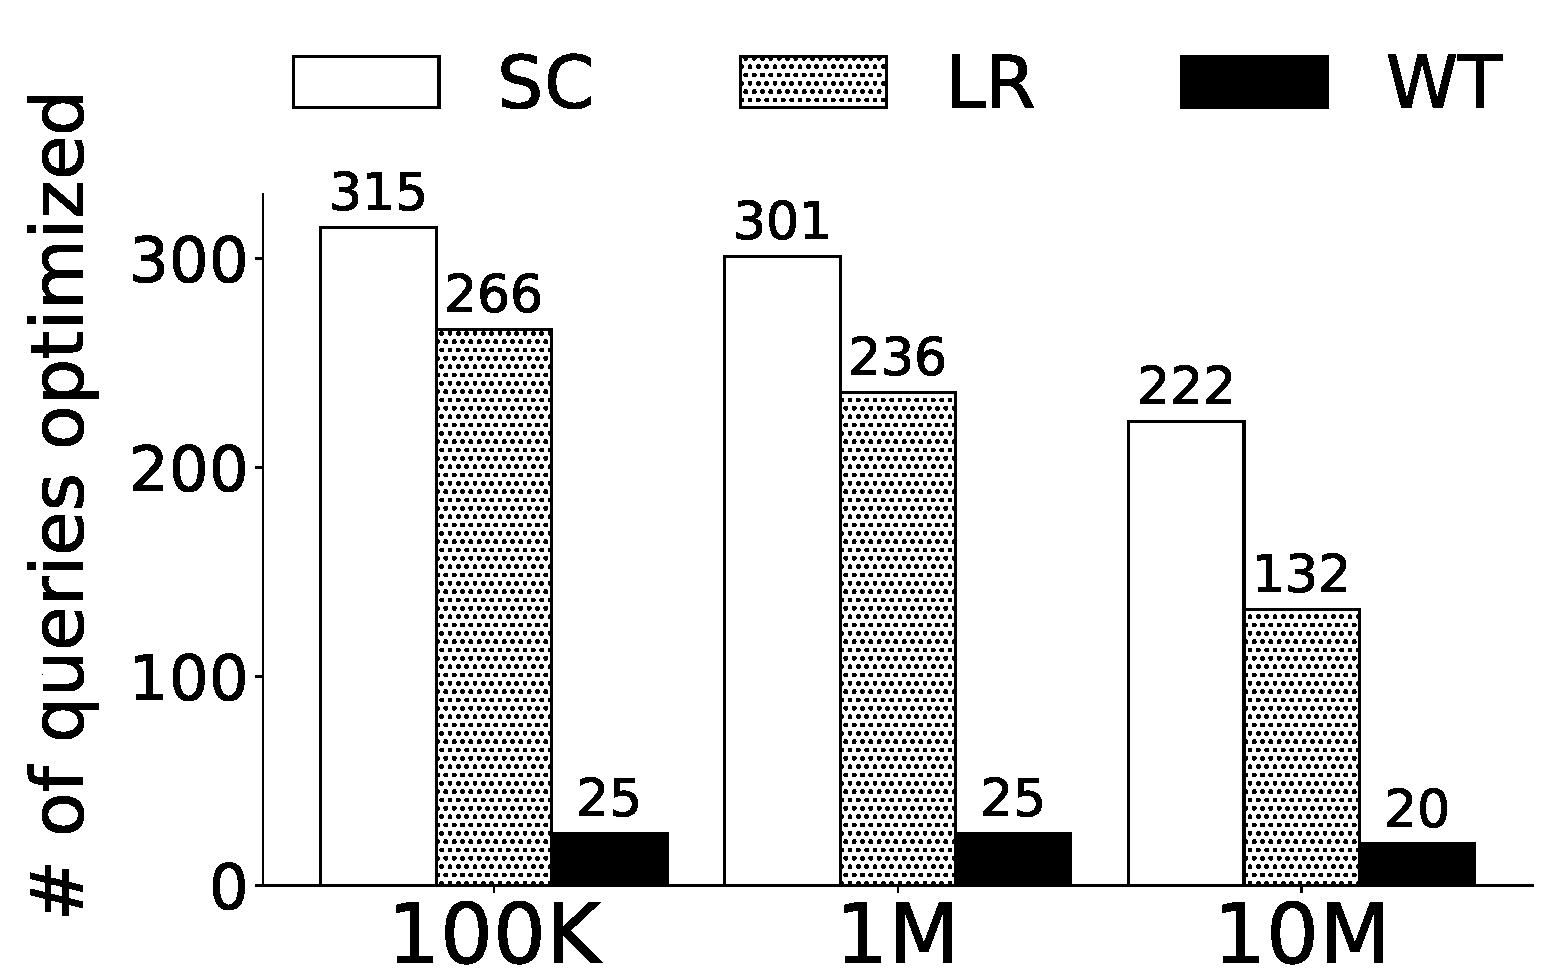
\includegraphics[width=\linewidth]{chapters/slabcity/figs/coverage_LeetCode_time.pdf}
\caption*{\small (a) Coverage (\# of queries).}
\label{slab:fig:leetcode-coverage}
\end{minipage}\hfill
\begin{minipage}[t]{.48\linewidth}\centering
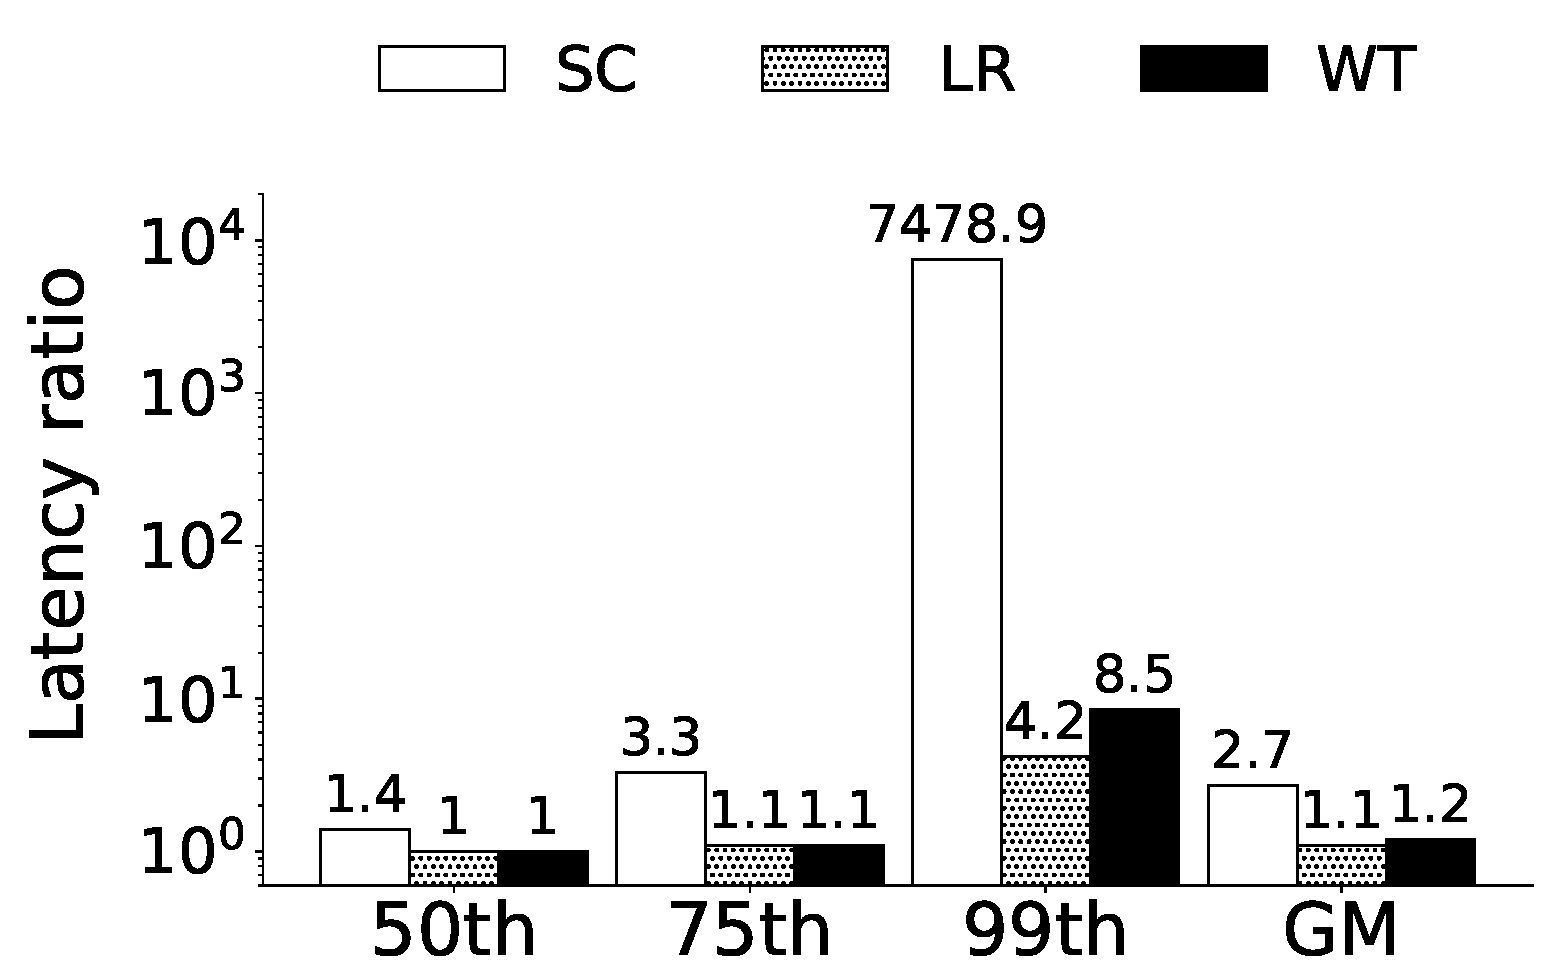
\includegraphics[width=\linewidth]{chapters/slabcity/figs/time_LeetCode_100K.pdf}
\end{minipage}\\[8pt]
\begin{minipage}[t]{.48\linewidth}\centering
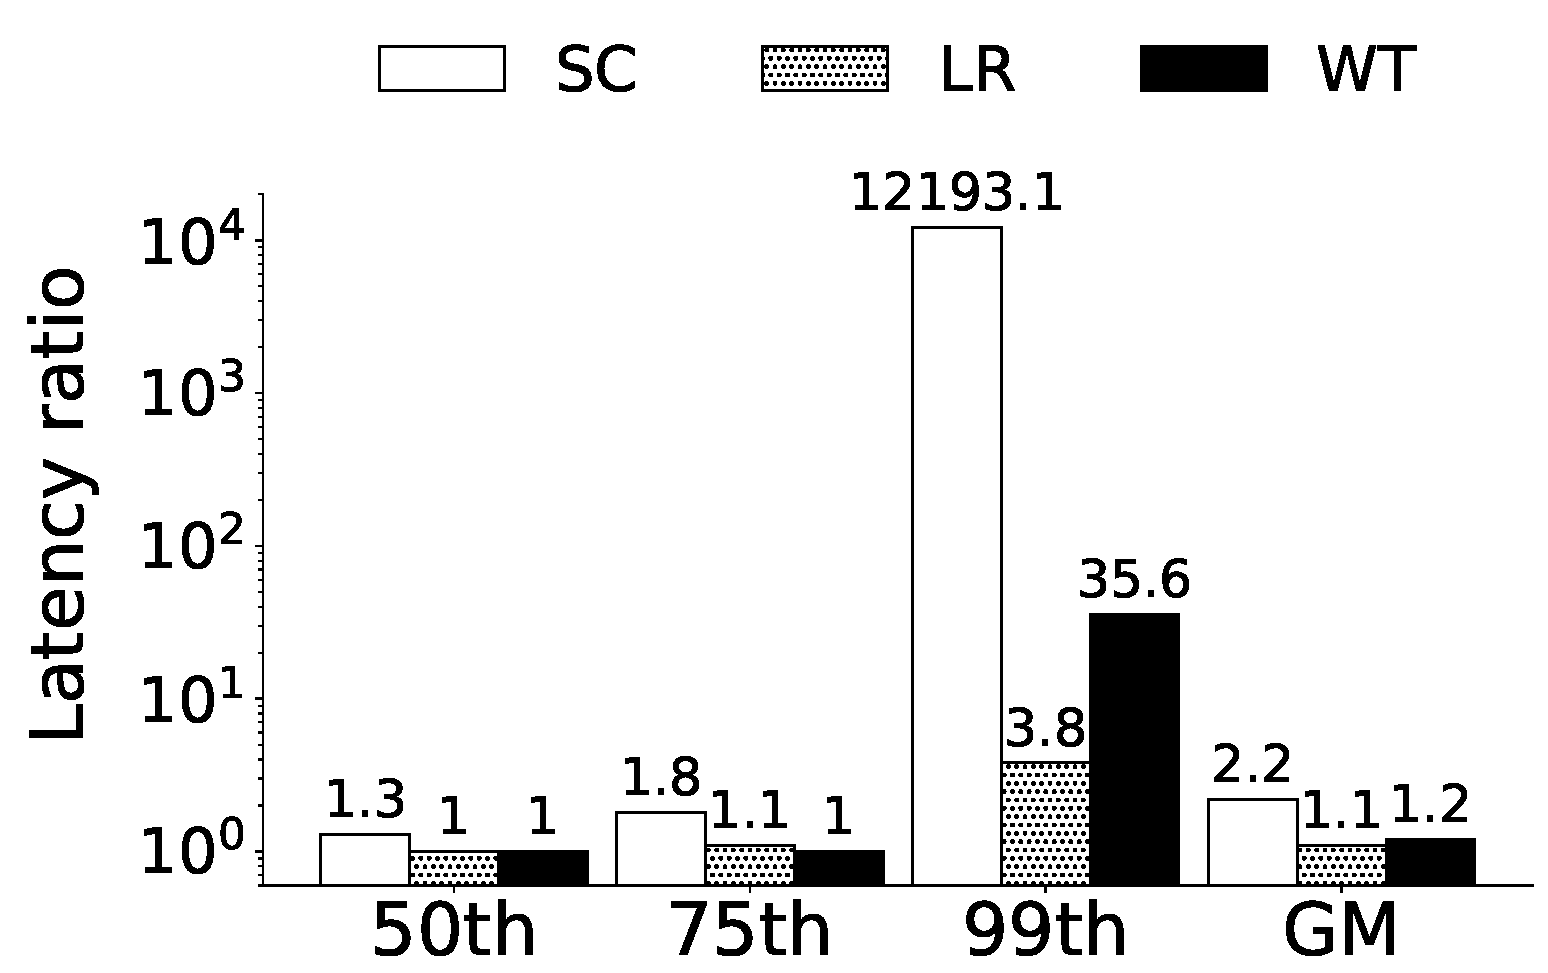
\includegraphics[width=\linewidth]{chapters/slabcity/figs/time_LeetCode_1M.pdf}
\end{minipage}\hfill
\begin{minipage}[t]{.48\linewidth}\centering
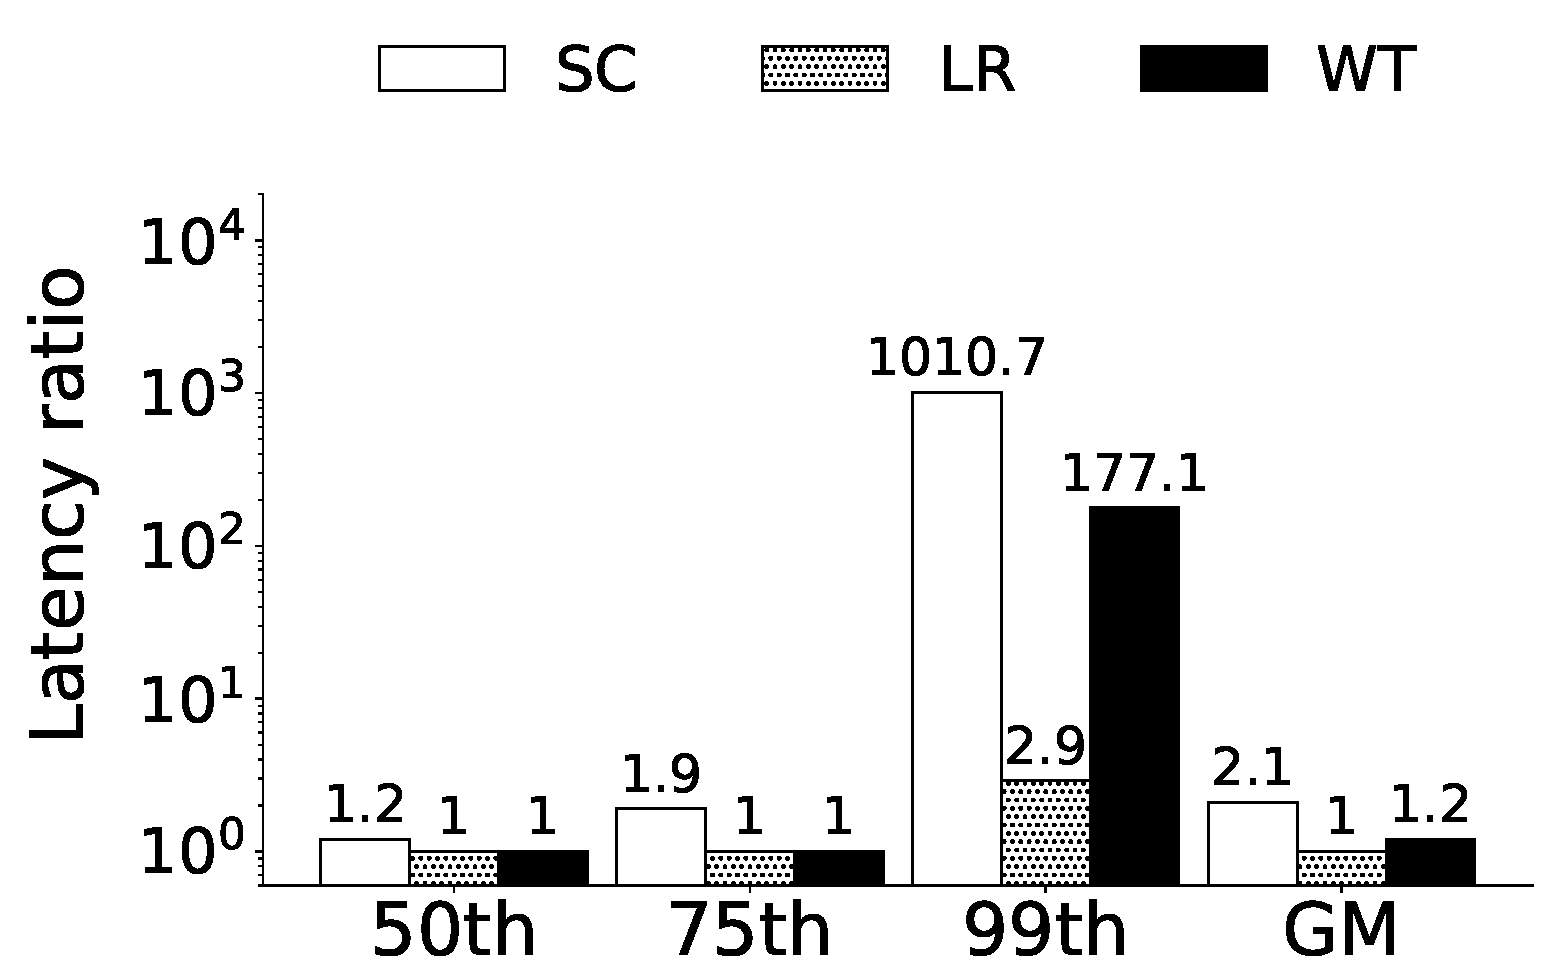
\includegraphics[width=\linewidth]{chapters/slabcity/figs/time_LeetCode_10M.pdf}
\end{minipage}
\caption*{\small (b) Latency reduction: top right is on 100K, bottom left is on 1M, and bottom right is on 10M. ``GM'' means geometric mean.}
\label{slab:fig:leetcode-reduction-latency}
\caption{\barzanrev{LeetCode results across all data sizes with uniform distribution.}}
\label{slab:fig:leetcode-results}
\end{figure*}




\begin{figure*}[!t]
\centering
% NOTE (dissertation): re-laid out from the paper's 1x4 strip to a 2x2 grid.
\begin{minipage}[t]{.48\linewidth}\centering
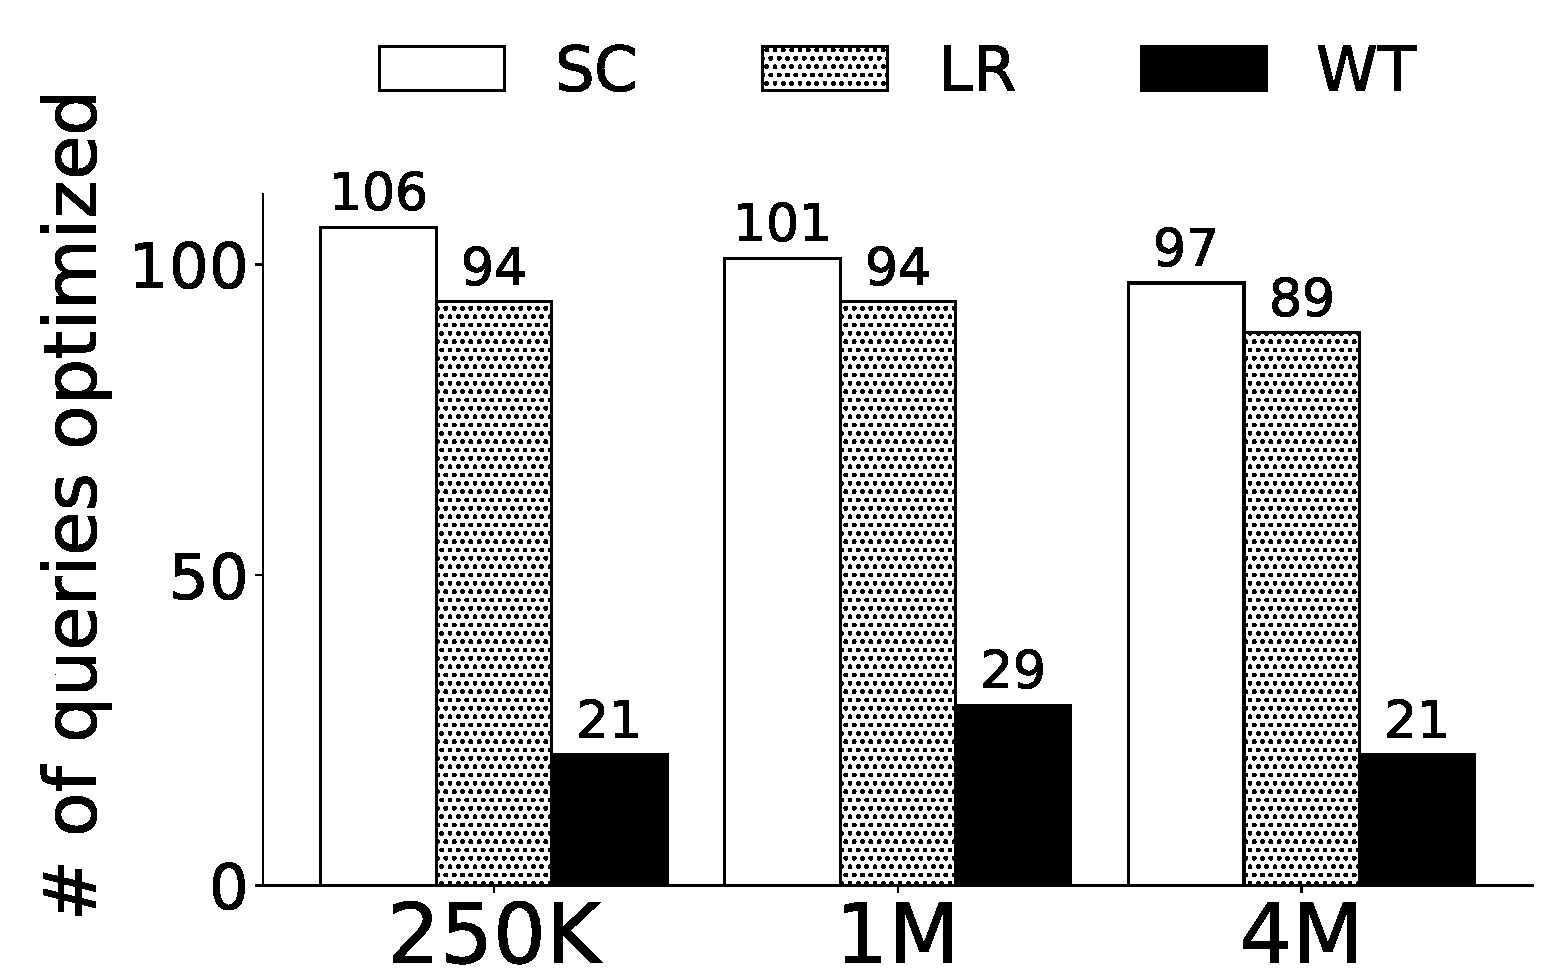
\includegraphics[width=\linewidth]{chapters/slabcity/figs/coverage_Calcite_time.pdf}
\caption*{\small (a) Coverage (\# of queries).}
\label{slab:fig:calcite-coverage}
\end{minipage}\hfill
\begin{minipage}[t]{.48\linewidth}\centering
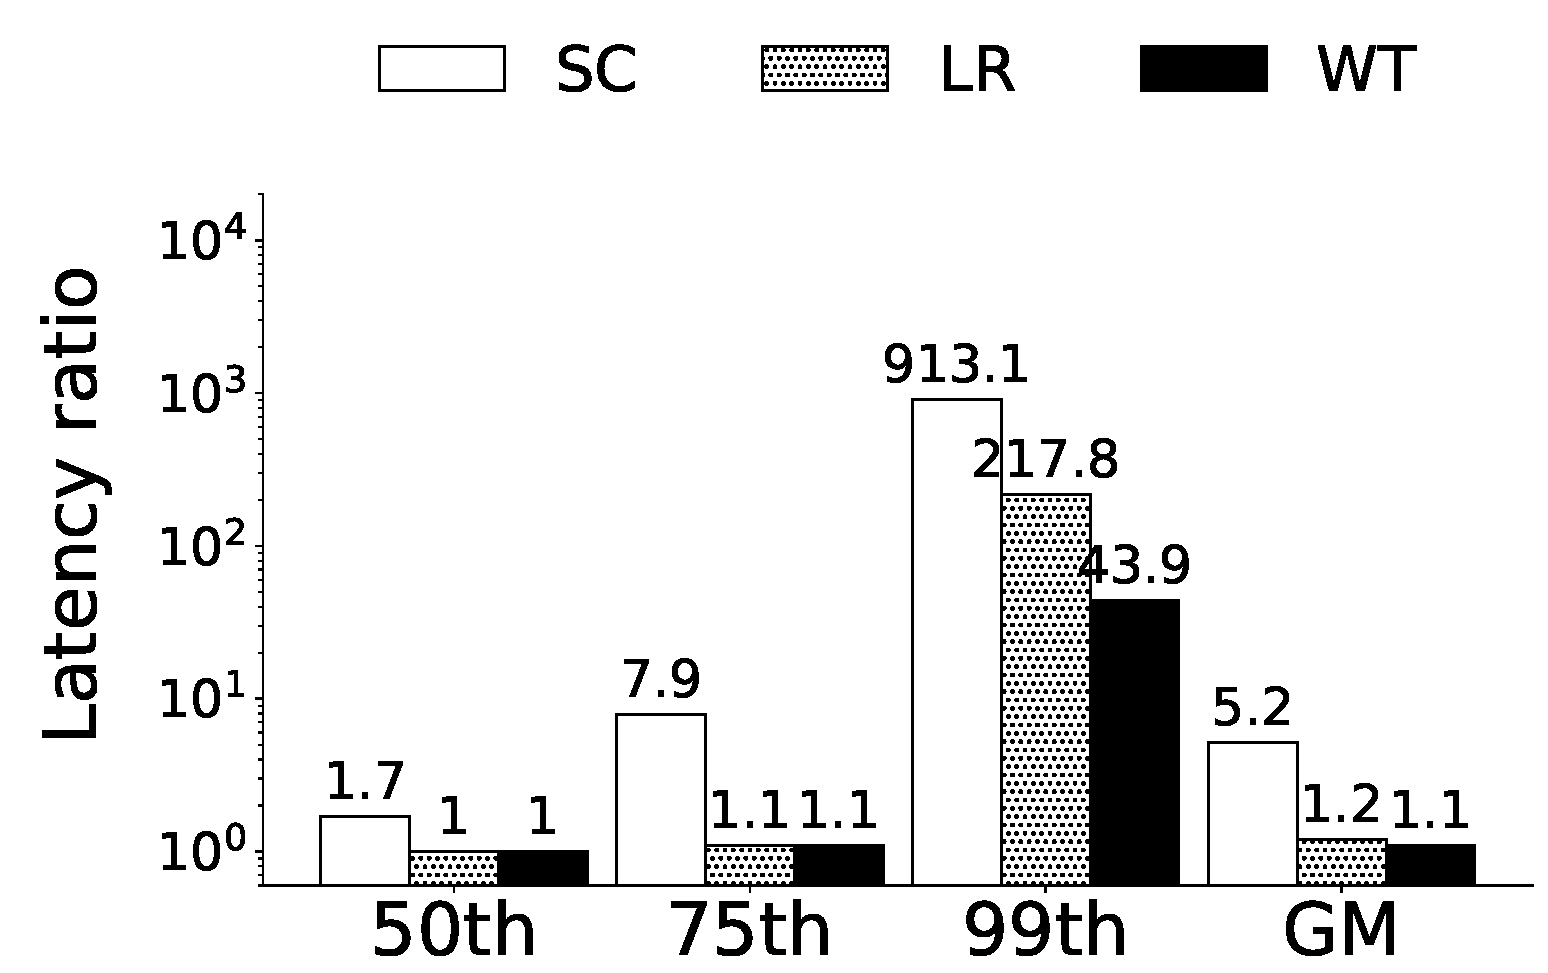
\includegraphics[width=\linewidth]{chapters/slabcity/figs/time_Calcite_250K.pdf}
\end{minipage}\\[8pt]
\begin{minipage}[t]{.48\linewidth}\centering
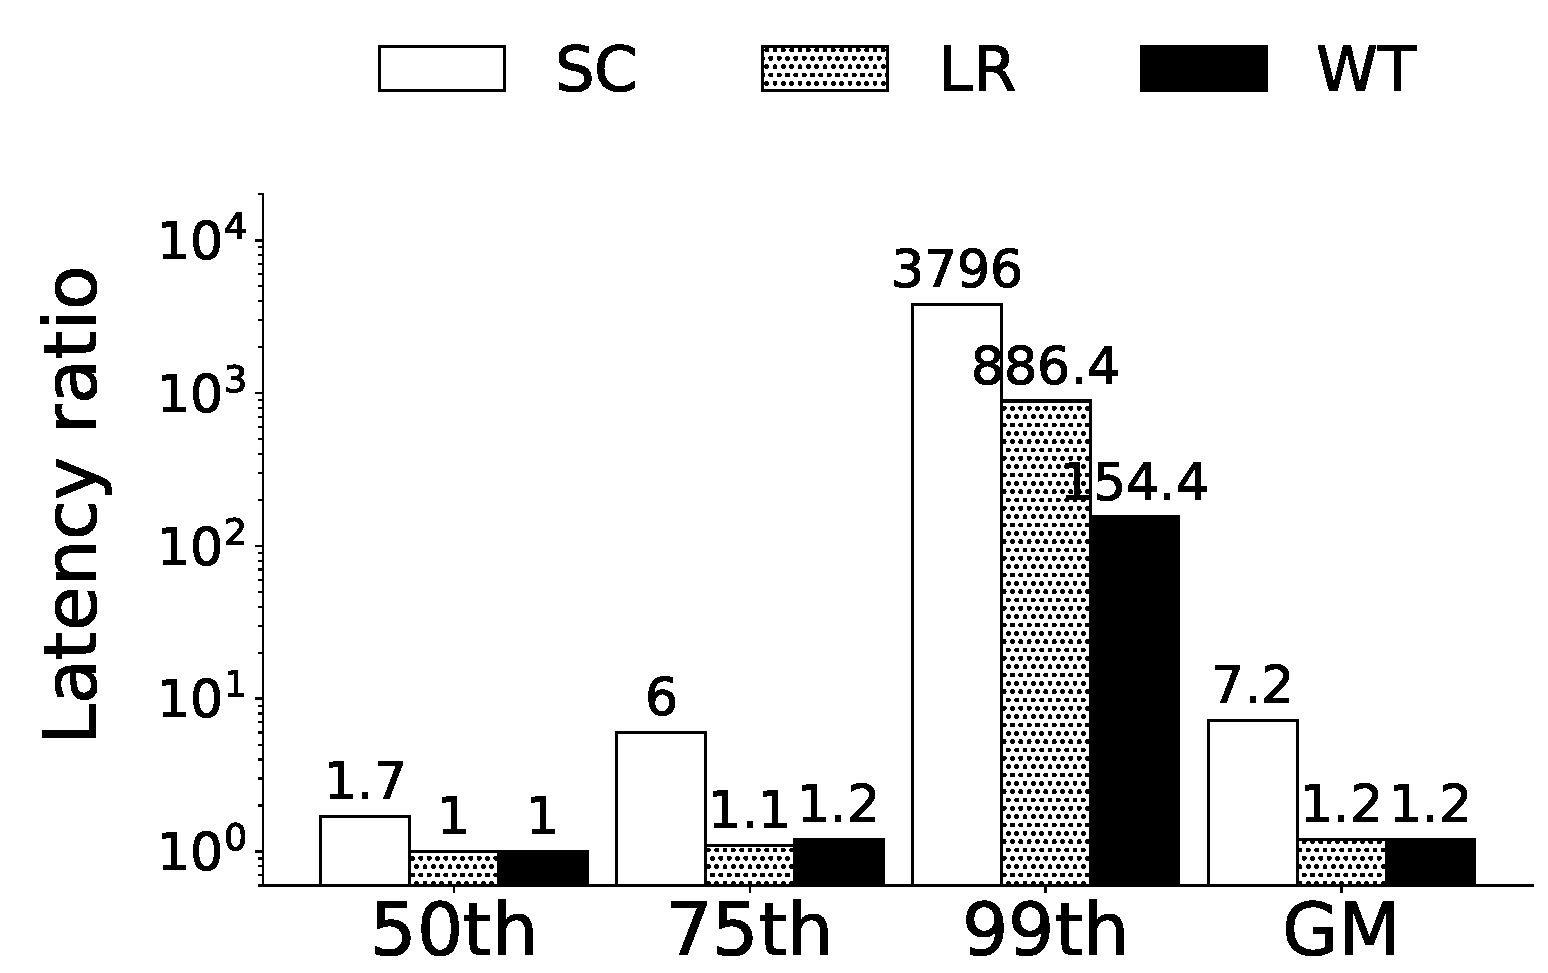
\includegraphics[width=\linewidth]{chapters/slabcity/figs/time_Calcite_1M.pdf}
\end{minipage}\hfill
\begin{minipage}[t]{.48\linewidth}\centering
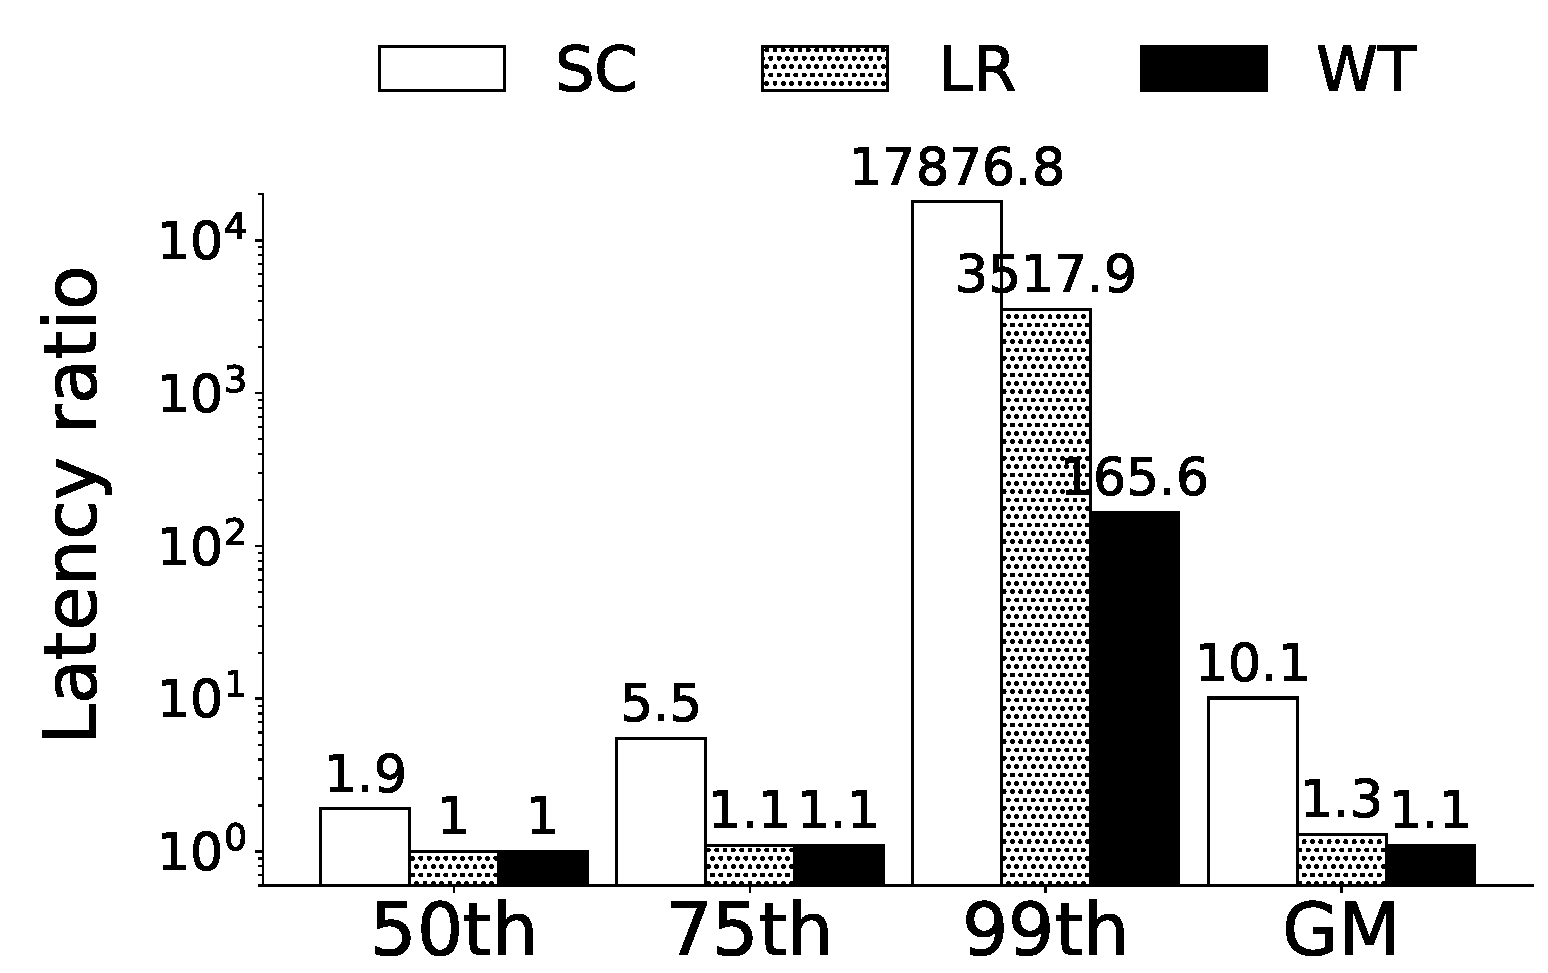
\includegraphics[width=\linewidth]{chapters/slabcity/figs/time_Calcite_4M.pdf}
\end{minipage}
\caption*{\small (b) Latency reduction: top right is on 250K, bottom left is on 1M, and bottom right is on 4M. ``GM'' means geometric mean.}
\label{slab:fig:calcite-reduction-latency}
\caption{\barzanrev{Calcite results across all data sizes with uniform distribution.}}
\label{slab:fig:calcite-results}
\end{figure*}




Our experiments are designed to answer the following questions:

\begin{itemize}[leftmargin=*]  \setlength\itemsep{2pt}
\item 
\textbf{Coverage:} 
How does $\toolname$'s \emph{coverage} compare against that of state-of-the-art query rewriting techniques? 
That is, which technique can optimize more queries? 
(Section~\ref{slab:sec:q1-coverage}) 
\item 
\textbf{Query latency reduction:}
How does $\toolname$ compare to state-of-the-art query rewriters in terms of the efficiency of the generated queries? 
That is, for input queries that can be rewritten, which technique leads to faster queries? 
(Section~\ref{slab:sec:q2-reduction})
 
\item
\textbf{Ablation study:} How important are various ideas in \slabcity? 
(Section~\ref{slab:sec:ablation})

\end{itemize}



\subsection{Experimental Setup}
%In what follows, we describe our workloads, data generation method, baselines, and experiment environment.

\head{Testbed}
All of our experiments (including running \toolname and baselines as well as executing queries) are conducted on Amazon EC2 r5.large instances,
% \barzan{is it EC2? if so then mention the size, eg. 2XL or something like that}
with 16GB RAM, 200GB gp2 SSD and Xeon E5-2686 v4 CPU running Ubuntu 22.04.
We use PostgreSQL 12.13.

\head{Workloads} 
{We use a wide range of different workloads:}
\begin{itemize}[leftmargin=*]
\item 
\textbf{LeetCode.} 
These are SQL queries, written by actual developers to solve different problems on LeetCode~\cite{leetcode}. 
Specifically, we first crawled \emph{all publicly available} SQL queries accepted by LeetCode as ``correct'' solutions. However, a number of them are actually incorrect due to missing tests on LeetCode. Hence, we manually filtered out as many incorrect queries as we could. 
In the end, we were left with a curated suite of 1131 queries overall. 
% Our dataset contains queries that solve a wide range of tasks (see some examples from Section~\ref{slab:sec:motivating-example}). 
%Then, we grouped these queries based on the LeetCode problem they are solving. 
%For each problem, we were left with dozens of correct queries that are all \emph{semantically equivalent} but \emph{syntactically distinct}.
Some of these solutions are poorly-written and therefore slow-running (which we hypothesize were authored by SQL novices) -- this makes  our LeetCode dataset especially 
valuable for evaluating query rewriting techniques. 
We also formalized the schemas and integrity constraints for all LeetCode tasks. 
%based on the description from the LeetCode website. 

\begin{comment}
\cancut{Overall, the queries were quite diverse and non-trivial. On our 10M database, \todo{xx} queries do not terminate within 10 hours, and \todo{xx} queries take at least \todo{xx} seconds to finish. Even on our smallest database with 100K rows, \todo{xx} queries take more than \todo{xx} seconds.}
\end{comment}



\item 
\textbf{Calcite.}
Our second workload is constructed from the Calcite's \emph{optimization rules} test suite~\cite{calcite-test-suite}, which is used in prior work~\cite{wetune} for evaluating query rewriting. We include all 794 queries. %in our experiments.
%The Calcite project also includes the schema and integrity constraints.


\item 
\barzanrev{\textbf{TPC.}
Finally, we also use queries from the standard TPC-H~\cite{tpc-h} and TPC-DS~\cite{tpc-ds} workloads.}
\end{itemize}


\head{Data generation} 
We generate large databases for each workload. 
For \leetcode, we use three data sizes (100K, 1M, and 10M). For \calcite, we use 250K, 1M, and 4M (4M is the largest data size that can fit in 16G memory). 
For both workloads, we follow prior work~\cite{wetune} and use \barzanrev{two different data distributions: uniform and Zipfian
% \barzan{isn't Zipfian capitalized everywhere?} \jie{also used in WeTune paper. And they also use the skewed parameter of 1.25. Do we need to mention it?}
(with a skewed parameter of 1.25, as used in \cite{wetune}).}
% \barzan{is 1.25 skeweed enough?} \jie{see above. Yes, I believe it is skewed enough}
We also make sure the generated data meets the integrity constraints. 
\barzanrev{For TPC-H and TPC-DS workloads, we use their official data generation script with the same scale factor as in $\learnedrewrite$~\cite{LR} (which is 1, meaning 1G data size).}





\head{Baselines}
We compare $\toolname$ against two state-of-the-art rule-based query rewriting techniques: 
\begin{itemize}[leftmargin=*]
\item
\textbf{\learnedrewrite} (or \LR, VLDB 2022~\cite{LR,LR-source-code}) is a state-of-the-art \emph{rule-based} query rewriter which uses Monte Carlo Tree Search to guide the rule-based rewriting process. In particular, \LR uses rewrite rules from \calcite and was shown to outperform multiple existing techniques from prior work~\cite{begoli2018apache,pirahesh1992extensible}.
\item 
\textbf{\wetune} (or \WT, SIGMOD 2022~\cite{wetune,WT-source-code}) is the state-of-the-art automated query rewrite rule generator. It had discovered dozens of new rules, previously missing from existing rule-sets. These new rules were shown to lead to new optimizations previously not considered by existing systems (such as MS SQL Server).  
\end{itemize}




\begin{comment}
\rui{All of our experiments are conducted on AWS EC2 
instances (r5.large type, with 16GB RAM, 200GB disk, Xeon E5-2686 v4 CPU, running Ubuntu 22.04 and PostgreSQL 12.13). We launched instances using the same Amazon Machine Image with testing databases loaded to ensure the same experiment setups over all instances. We collected cost by first running VACUUM ANALYZE and running EXPLAIN on queries on a single machine. For the running time, we partitioned the queries to collect their running time on multiple instances parallelly. For LeetCode experiments, we partitioned queries using problem ID so that all queries corresponding to the same problem id are run on the same instance. For Calcite experiments, we ensured that outputs that correspond to the same test were run on the same instances.  Between each run, we restarted the PostgreSQL service and cleared the cache.}
\end{comment}





%ta inja

\subsection{Coverage}
\label{slab:sec:q1-coverage}

This section reports the number of queries from each workload that \toolname can optimize, and compare it with baselines.


\head{Setup}
Given each query $\inputquery$ (and the corresponding schema) from each workload, we run \toolname (using a 5-second timeout) and obtain an output query $\query$. 
Then, we check whether or not $\query$ indeed optimizes $\inputquery$ in terms of latency: if $\query$ has a smaller latency than $\inputquery$, we say $\query$ optimizes $\inputquery$. 
%\barzan{this def should  come much earlier in the paper} %\xinyu{I added this to section 2.}
%Similarly, $\query$ optimizes $\inputquery$ in terms of latency, if $\query$ has a smaller execution time than $\inputquery$. 
We run each query (both input and rewritten queries) 3 times and take their average as the final latency value.
%the first run serves as warm-up whereas the average of the next 3 runs is used as the final latency value. 
Before each run, we restart the PostgreSQL service and clear the database cache. 
We use 10 hours as the timeout; output queries that do not terminate before timeout are marked as ``not optimized''. 
The same setup is used for the baselines. 

\vspace{5pt}
\evalfinding{\emph{\toolname can optimize more queries across different workloads.}}




\begin{table}[!t]
%\small 
\footnotesize
\caption{\barzanrev{\small LeetCode and Calcite results with Zipfian distribution.}}
\vspace{-8pt}
\centering
\setlength{\tabcolsep}{2pt}
\def\arraystretch{1.1}
\begin{tabular}{  c | r r r | r r r | r r r | r r r }
\toprule
& \multicolumn{6}{c|}{Coverage (\# of queries)} 
& \multicolumn{6}{c}{Latency ratio (geometric mean)} 
\\ 
\midrule
& \multicolumn{3}{c|}{LeetCode} 
& \multicolumn{3}{c|}{Calcite} 
& \multicolumn{3}{c|}{LeetCode} 
& \multicolumn{3}{c}{Calcite} 
\\ 
& 100K & 1M & 10M 
& 250K & 1M & 4M 
& 100K & 1M & 10M 
& 250K & 1M & 4M 
\\ 
\midrule
$\toolname$
& \textbf{318} & \textbf{269} & \textbf{186}
& {\textbf{101}} & {\textbf{99}} & {\textbf{96}}
& \textbf{3.1x} & \textbf{2.7x} & \textbf{2.2x}
& {\textbf{5.4x}} & {\textbf{8.8x}} & {\textbf{12.8x}}
\\ 
$\LR$
& 262 & 243 & 154  
& {95} & {94} & {86} 
& 1.1x & 1.2x & 1x
& {1.2x} & {1.3x} & {1.3x}

\\ 
$\WT$
& 24 & 23 & 24  
& {20} & {23} & {18}
& 1.4x & 1.6x & 1.6x
& {1.2x} & {1.2x} & {1.2x}
\\ 
\bottomrule
\end{tabular}
%\vspace{5pt}

\label{slab:tab:zipfian-results}
\vspace{-15pt}
\end{table}




\head{Results}
Figure~\ref{slab:fig:leetcode-results}(a) and Figure~\ref{slab:fig:calcite-results}(a) present the coverage results for all techinques (including $\toolname$ and baselines) across LeetCode and Calcite workloads (using a uniform distribution). 
For example, looking at Figure~\ref{slab:fig:leetcode-results}(a), for 10M, \toolname can optimize 222 input queries, whereas $\learnedrewrite$ and $\wetune$ can only 
optimize 132 and 20 queries, respectively. 
\barzanrev{We also note that since $\toolname$'s checker can fully verify only a subset of its output queries, we manually inspected all the remaining queries that only pass the tester and bounded verifier (see Section~\ref{slab:sec:eval:discussion} for a detailed discussion on the limitation of full verification) and confirmed the optimizations included in our results are indeed correct} (i.e., all input-output query pairs are equivalent).
%\barzanrev{Although the checker can offer full verification for only a subset of the output queries, we manually inspect and confirm all our optimizations are indeed correct} (i.e., all input-output query pairs are equivalent). 
\barzanrev{For the Zipfian distribution, we obtain similar results, as shown in Table~\ref{slab:tab:zipfian-results}.}
Overall, $\toolname$ significantly outperforms existing rule-based systems, highlighting the superiority of a whole-query synthesis-based approach.


\barzanrev{For the TPC-H workload, $\toolname$ is able to optimize 2 (out of 22) input queries (\#17 and \#20) in less than 5 seconds. $\LR$ is able to optimize the same two queries, while $\WT$ cannot optimize any.
The TPC-DS queries are far more complex, but $\toolname$ can still optimize three queries (\#1, \#30 and \#81) within 5 seconds. $\LR$ can optimize two (\#1, \#30) but $\LR$'s output queries are much slower than $\toolname$'s. Again, $\WT$ is not able to optimize any.}



\head{Discussion}
The gap between \toolname's coverage and baselines' on LeetCode is much higher than that on Calcite: we believe this highlights the usefulness of our LeetCode dataset and the advantage of our synthesis-based technique over rule-based ones in optimizing new query patterns. 
In particular, LeetCode has more queries that are larger and use more aggregation and window functions than those in Calcite. 
\barzanrev{While $\toolname$'s coverage is considerably higher than all baselines, there are still 
some queries covered by baselines and not covered by $\toolname$.
%While rare (\todo{??\% for)}, 
Some of these queries involve operators (e.g., coalesce) that are not yet supported by our prototype. 
Another reason has to do with our 5s timeout. 
Our plan for future improvement of our prototype (e.g., supporting more operators and optimizing the performance such as by parallelizing the search) should help with both reasons.}
%Another reason is our 5s timeout. 
%Our plans for future improvement of our implementation (supporting more operators and improving the efficiency) should help with both reasons.}





\begin{comment}
    

\todo{if above looks good, we can comment out below. }
\jierevision{There are two primary explanations as to why our tool may be unable to optimize for certain queries, while baselines can. The first reason is that baselines rewrite the input query by employing operators (e.g., $\sqlcoalescecolor$) that are not available in our DSL. The second reason is that sometimes our score function fails to capture the similarity in semantics of different dataflows and hence assigns some promising candidates with lower scores than expected. As a result, they cannot be found within 5s timeout. Table~\ref{slab:tab:Q11-Q12} shows queries finding the team size of each employee. \slabcity did not capture the relationship between $\sqloncolor \ e1.team = e2.team$ and $\sqlgroupbycolor \ team$ and failed to find the optimal query. To address this issue, one solution is to adjust the score function to take this relationship into account. However, it is important to note that incorporating more dataflows will inevitably lead to increased search time, which is a tradeoff that needs to be carefully balanced.} 

\begin{table}[!t]
\small 
\begin{tabular}{|c|c|}
\hline
 $\query_{11}$

 & 
  % \\
  %             \hspace{2em} 
 \makecell[l]{\sqlselectcolor \  e1.employee\_id, \sqlcountcolor(e2.employee\_id) \sqlascolor s\\
              \sqlfromcolor employee \sqlascolor e1 \sqljoincolor employee \sqlascolor e2 \sqloncolor e1.team = e2.team\\
              $\sqlgroupbycolor$ e1.employee\_id
              }  
\\
\hline
$\query_{12}$
&
 \makecell[l]{ \sqlselectcolor e1.employee\_id, e2.s, \\ \sqlfromcolor employee \sqlascolor e1 \sqljoincolor \\
 \hspace{0.5em} (\sqlselectcolor team, \sqlcountcolor(*) \sqlascolor s \sqlfromcolor employee \sqlgroupbycolor \ team) \sqlascolor e2 \\ \hspace{0.5em} \sqloncolor e1.team = e2.team}
 
  \\
 \hline
\end{tabular}
\vspace{5pt}
\caption{\jierevision{$\query_{11}$ is human-written. $\query_{12}$ is the optimal form.}}
\vspace{-20pt}
\label{slab:tab:Q11-Q12}
\end{table}

\end{comment}


\subsection{Query Latency Reduction}
\label{slab:sec:q2-reduction}


In this section, we compare the performance of queries synthesized by $\toolname$  with those generated by (rule-based) baselines. Higher coverage (Section~\ref{slab:sec:q1-coverage}) means $\slabcity$ can optimize more queries, 
but does it also lead to better (i.e., faster) queries than baselines?

\head{Setup}
We use the same setup as in Section~\ref{slab:sec:q1-coverage} and measure the reduction ratio in query latencies across each technique's output queries. 
For example, given $\inputquery$ and its corresponding output query $\query$ synthesized by \toolname, a latency reduction of 5x means $\query$ is 5x faster than $\inputquery$. 
We still use 10 hours as the timeout --- in case of a timeout, we use 10 hours as the latency; however, if both $\inputquery$ and $\query$ time out, we do not include this data point. 
%Latency reduction ratios for baselines are measured in the same way.

\vspace{5pt}
\evalfinding{\emph{\toolname generates faster queries across different workloads.}}


\head{Results}
We present the latency reduction results for LeetCode and Calcite workloads (using a uniform distribution) in Figure~\ref{slab:fig:leetcode-results}(b) and Figure~\ref{slab:fig:calcite-results}(b). 
For example, looking at Figure~\ref{slab:fig:leetcode-results}(b), for 10M (rightmost figure), on average, $\toolname$ achieves a 50.3x latency reduction ratio \emph{across all output queries}, whereas $\LR$ is 1.4x and $\WT$ is 12x. 
\barzanrev{We also report additional statistics: median (50th) and 75th percentiles.}
As we can see, $\toolname$ always outperforms baselines by a significant margin across both workloads and for all data sizes. 
\barzanrev{For output queries that can be covered (i.e., optimized) by $\toolname$,} the median is as high as 1.9x for LeetCode and 2.2x for Calcite.
% \barzan{what does it mean for median to be up to? shouldn't median be a single number?
% maybe we can reword to `as high as` instead of up to}
% \xinyu{because we have multiple data sizes.}
% \barzan{the following is confusing: we say on the other hand if we said on the one hand earlier which we didn't early. what are we trying to say in the next sentence? } \xinyu{we can remove OTOH}
% On the other hand, 
\barzanrev{For the Zipfian distribution, $\toolname$ also outperforms all baselines; see Table~\ref{slab:tab:zipfian-results} for more details.}

\barzanrev{For TPC-H, $\toolname$ and $\LR$ achieve similar latency speed-ups (both by more than an order of magnitude). 
For TPC-DS, $\toolname$ can optimize one query that $\LR$ is not able to optimize. For the two TPC-DS queries that both can optimize, $\toolname$ outputs faster queries compared to $\LR$'s. For all three TPC-DS queries, $\toolname$ can speed-up the original queries by at least one order of magnitude.}

%\xinyurevision{\todo{For TPC-H, $\toolname$ and $\LR$ produce queries with very similar latency reduction ratios. However, for TPC-DS, $\toolname$'s output queries are significantly faster. In particular, it achieves a {1034x} reduction for query \#1 and $\LR$ is {189x}. For \#30, $\toolname$ is {113x} and $\LR$ is {26x}. \ruirevision{For \#81, $\toolname$ is 364x and $\LR$ can not optimize.}}}


{\head{Discussion}
Similar to Section~\ref{slab:sec:q1-coverage}, \toolname's margins of improvement on LeetCode are even more significant than on Calcite, which we believe is due to the same reasons mentioned earlier: 
existing rule-based systems and \learnedrewrite's rule-set are specifically designed based on Calcite queries and LeetCode is a useful dataset to evaluate query rewriters. 
Careful readers may observe that \toolname's reduction on LeetCode 10M is lower than that on 1M.
This is due to 15 input queries (all from problem \#1308) which do not terminate within 10 hours on both sizes. Surprisingly, \toolname is able to optimize these queries: the fastest output query terminates in 3 seconds on 1M but takes more than 30 seconds on 10M. 
As we used 10 hours as the latency for the timed-out input query in both cases, this makes the reduction on 10M lower than that on 1M.}




\begin{table}[!t]
%\small 
\footnotesize
\caption{\small Time breakdown on average and other statistics.}%Bottom:  other statistics (e.g., the average number of queries enumerated).}
\vspace{-8pt}
\centering
\setlength{\tabcolsep}{3pt}
\def\arraystretch{1.5}
\begin{tabular}{  R{180pt} | r  r   }
\toprule
\% of time spent on 
& LeetCode
& Calcite
%& TPC-H 
%& TPC-DS 
\\ \midrule
{query search (line~\ref{slab:alg:toplevelalg:forloop})} 
& {37.4\%}
& {6.9\%} 
%& \ruirevision{48.0\%}
\\ 
{checking against counterexamples (line~\ref{slab:alg:toplevelalg:satisfycounterexample}}) 
& {10.8\%}
& {0.9\%}
%& \ruirevision{2.9\%}
\\ 
{equivalence  checking (line~\ref{slab:alg:toplevelalg:checkequiv}})
& {51.4\%}
& {92.2\%}  
%& \ruirevision{51.0\%}
\\ 
%\emph{\% of time on testing} 
%& 32.6\% 
%& 65.5\% 
%\\ 
%\emph{\% of time on verification} 
%& 23.6\% 
%& 31.6\% 
%\\ \midrule 
{performance ranking (line~\ref{slab:alg:toplevelalg:checkfaster})} 
& {0.4\%} 
& {0.1\%} 
%& \ruirevision{0.1\%}
\\ \midrule \midrule 
{avg \# of queries enumerated}
& {437} 
& {104}
%& \ruirevision{216}
\\ 
{avg \# of counterexamples generated}
& {1.4}
& {1.2}
%& \ruirevision{1}
\\ 
{avg \# of equivalent queries synthesized}
& {66}
& {15} 
%& \ruirevision{32}
\\ \bottomrule
\end{tabular}

\vspace{-12pt}
\label{slab:tab:time-breakdown}
\end{table}




\subsection{Detailed Analysis and Ablation Study}
\label{slab:sec:ablation}

%In this section, we analyze the time that is spent on different steps of \slabcity. We also perform a few ablation studies to measure the impact of various design decisions we have made in \slabcity.


\begin{comment}
    

\begin{table}[!t]
%\small 
\footnotesize
\centering
\setlength{\tabcolsep}{2pt}
\def\arraystretch{1.1}
\begin{tabular}{  c | r r | r r  }
\toprule
& \multicolumn{2}{c|}{LeetCode} 
& \multicolumn{2}{c}{Calcite} 
%& \multicolumn{2}{c|}{TPC-H} 
%& \multicolumn{2}{c}{TPC-DS} 
\\ 
& median 
& max 
& median 
& max 
%& median 
%& max 
%& median 
%& max 
\\ 
\midrule
$\toolname$
& {0.84} & {4.84} & 
 {0.74}	&  {4.81}	
 %& \ruirevisiontbd{4.15}  &  \ruirevisiontbd{4.58}	 &  \ruirevisiontbd{5.03}		& \ruirevisiontbd{5.74}
\\ 
$\learnedrewrite$
& 0.03 & 0.73 & 0.25	& 3.75	 
%& 0.25 & 	1.58 & 	2.48	& 25.51 
\\ 
$\wetune$
& 0.24	& 0.46 &	0.001	& 0.17	
%& 0.36	& 0.36	& NA &	NA 
\\ 
\bottomrule
\end{tabular}
%\vspace{5pt}
\caption{{\small Running time statistics to generate rewrites (in seconds). For $\toolname$, we report the time when an output query (synthesized using 5-second timeout) is found.}}
\label{slab:tab:running-time-stats}
\vspace{-20pt}
\end{table}

\end{comment}



\begin{table}[!t]
\centering
\footnotesize
\centering
\setlength{\tabcolsep}{6pt}
\def\arraystretch{1.5}
\caption{\small Running time statistics to generate rewrites (in seconds).For $\toolname$, we report the time when an output query (synthesized using 5-second timeout) is found.}
\vspace{-5pt}
\begin{tabular}{  c | r r | r r  }
\toprule
& \multicolumn{2}{c|}{LeetCode} 
& \multicolumn{2}{c}{Calcite} 
%& \multicolumn{2}{c|}{TPC-H} 
%& \multicolumn{2}{c}{TPC-DS} 
\\ 
& median 
& max 
& median 
& max 
%& median 
%& max 
%& median 
%& max 
\\ 
\midrule
$\toolname$
& {0.84} & {4.84} & 
 {0.74}	&  {4.81}	
 %& \ruirevisiontbd{4.15}  &  \ruirevisiontbd{4.58}	 &  \ruirevisiontbd{5.03}		& \ruirevisiontbd{5.74}
\\ 
$\learnedrewrite$
& 0.03 & 0.73 & 0.25	& 3.75	 
%& 0.25 & 	1.58 & 	2.48	& 25.51 
\\ 
$\wetune$
& 0.24	& 0.46 &	0.001	& 0.17	
%& 0.36	& 0.36	& NA &	NA 
\\ 
\bottomrule
\end{tabular}

\label{slab:tab:running-time-stats}
\end{table}

\begin{table}[!t]
% 
%
\centering
\footnotesize
\centering
\setlength{\tabcolsep}{2pt}
\def\arraystretch{1.1}
\caption{{\small Coverage (\# of queries) and geometric mean of latency reduction: using \texttt{EXPLAIN} vs. using exact latencies.}}
\vspace{-5pt}
\begin{tabular}{  c | r r r | r r r | r r r | r r r }
\toprule
& \multicolumn{6}{c|}{Coverage (\# of queries)} 
& \multicolumn{6}{c}{Latency ratio (geometric mean)} 
\\ 
\cmidrule{2-13}
& \multicolumn{3}{c|}{LeetCode} 
& \multicolumn{3}{c|}{Calcite} 
& \multicolumn{3}{c|}{LeetCode} 
& \multicolumn{3}{c}{Calcite} 
\\ 
& 100K & 1M & 10M 
& 250K & 1M & 4M 
& 100K & 1M & 10M 
& 250K & 1M & 4M 
\\ 
\midrule
w/ \texttt{EXPLAIN} 
& 315 & 301 & 222  & 106 & 101 & 97 
& {2.7x} & {2.2x} & {2.1x}  & {5.2x} & {7.2x} & {10.1x} 
\\ 
w/ exact latencies 
& {401} & {373} & {351}  & {121} & {117} & {112} 
& {2.9x} & {2.6x} & {2.2x}  & {4.8x} & 6.7x & {10.4x} 
\\ 
\bottomrule
\end{tabular}

\label{slab:tab:exact-latencies}
\end{table}


\head{Time breakdown}
Table~\ref{slab:tab:time-breakdown} shows the breakdown of how much time on average \toolname spends in each component (such as search and equivalence checking) and other statistics (such as the average number of queries generated during synthesis). 
In general, query equivalence checking (including both testing and verification) takes the majority of the time. 


\barzanrev{\head{Synthesis efficiency}
While $\toolname$ uses a 5s \emph{timeout}, many of its output queries are discovered 
much earlier.
Specifically, {58\%} of its output queries (generated using 5s timeout) are found within {1} second. 
In the words, the actual synthesis time to find the output query is shorter. 
Table~\ref{slab:tab:running-time-stats} presents the median and max of $\toolname$'s actual synthesis time for LeetCode and Calcite queries that $\toolname$ can rewrite.
As expected, rule-based approaches are generally faster, though $\LR$'s max time on Calcite is much slower. 
For TPC-H and TPC-DS, $\toolname$ takes 4-5 seconds for all queries it can optimize.}
%\xinyurevision{In comparison, $\LR$  is significantly slower: it takes up to 25 seconds for TPC-DS.}}














\begin{comment}

===== 
\xinyu{below is old stuff, but once we have Table 6 filled, will move something from below to above..}

As we can see, query testing takes more than 60\% of the total time, while verification takes more than 30\%. 
Note that this is not because our tester is slower than the verifier, but rather because the tester is run before verifier and disproved many inequivalent queries before they were sent to the verifier. 
For instance, on LeetCode 10M, an average of \rui{do you mean counter examples can not reject?} queries were sent to our tester, out of which only a dozen \rui{14.22} of queries were not disproved. 
On the other hand, our query search component tends to be quite fast. In particular, for LeetCode 10M, on average, a total of \rui{93 our algorithm ensures these queries are syntactically different and grammarly correct, so the number here is small, but high quality} queries can be searched within the 5-second time limit. Using \texttt{EXPLAIN} to collect cost estimates takes no time, since eventually only a handful of equivalent queries were synthesized --- e.g., for LeetCode 10M, on average, \rui{13.59} queries were ranked. 
\end{comment}



\begin{comment}


\begin{table}[!t]
\small 
\centering
\setlength{\tabcolsep}{3pt}
\def\arraystretch{1.2}
\begin{tabular}{ | r | c c c | c c c | }
\hline 
& \multicolumn{3}{c|}{LeetCode} 
& \multicolumn{3}{c|}{Calcite} 
\\ 
& 100K & 1M & 10M 
& 250K & 1M & 4M 
\\ \hline 
\emph{Query Search}
& 5.3\% & 5.4\% & 5.2\% & 0.7\% & 0.9\% & 0.9\%
\\ 
\emph{Equivalence Testing} 
& 61.4\% & 60.0\% & 60.3\%  & 66.1\% & 67.0\% & 67.3\%\\ 
\emph{Equivalence Verification} 
& 33.0\% & 34.3\% & 34.2\%  & 33.0\% & 32.0\% & 31.7\%\\ 
\emph{Performance Ranking} 
& 0.3\% & 0.3\% & 0.3\%  & 0.1\% & 0.1\% & 0.1\%
\\ \hline 
\end{tabular}
\vspace{5pt}
\caption{$\toolname$ time breakdown.}
\label{slab:tab:time-breakdown}
\end{table}

\end{comment}


\head{Impact of CEGIS}
How beneficial is the use of CEGIS? That is, if we do not re-use counterexamples when disproving queries, how inefficient would \toolname become? 
%In general, program synthesis is known to be prohibitively slow without using counterexamples~\cite{solar2008program}. To validate this in the context of synthesis-based query rewriting, 
%For instance, 
For LeetCode, with CEGIS, on average, $\toolname$ can search {437} queries in 5 seconds, where {1.4} counterexamples are generated; however, without re-using these examples, it can only search 175 queries on average within the same amount of time. 
This is because the tester spends extra time generating new counterexamples which are later dropped, but clearly they can be re-used to disprove other queries.  
This validates the observation made in prior work that CEGIS helps boost efficiency~\cite{solar2008program}. 

%generate \tofix{the examples from scratch.}\barzan{can we instead say `to disprove the same queries'?}
%This validates the observation made in other domains that CEGIS is critical for synthesis efficiency~\cite{solar2008program}. 




\head{Impact of query testing}
It is critical to reduce the frequency of invoking query verification. 
For instance, for LeetCode, on average our tester can disprove several dozens of queries within 1 second, whereas the verifier typically can handle at most a couple of queries within the same amount of time.
%A variant of \slabcity that invokes the query verifier to disprove \emph{every} candidate query (rather than always running the tester first)


\head{Impact of using dataflows to guide search}
A variant of $\slabcity$ that uses a naive search algorithm (that enumerates queries based on query size) was not able to optimize any of our input queries within 5 seconds. 
This highlights the importance of using dataflows to significantly accelerate query synthesis. 

\head{Impact of using cost estimates for ranking}
\texttt{EXPLAIN} is known to give inaccurate cost estimates. 
We study a variant of \slabcity where, instead of \texttt{EXPLAIN}, we  use the actual latency for each query (by running it against the database). 
While this variant is clearly impractical, it helps us understand how much \slabcity could be improved if we had access to a perfect predictor that could give the exact latency values. 
Table~\ref{slab:tab:exact-latencies} compares $\toolname$ w/ exact latency against our current $\toolname$ w/ \texttt{EXPLAIN} in terms of coverage; Table~\ref{slab:tab:exact-latencies} compares them in terms of latency reduction. 
In general, using exact latencies yields slightly higher coverage and latency reduction ratios, which is expected as that is the perfect predictor. 
However, we notice that using \texttt{EXPLAIN} to estimate query latency gives very close results and we believe this is a reasonable trade-off. 



\begin{comment}
    

\begin{table}[!t]
\footnotesize
\centering
\setlength{\tabcolsep}{3pt}
\def\arraystretch{1.1}
\begin{tabular}{  c | rrr | rrr  }
\toprule
& \multicolumn{3}{c|}{LeetCode} 
& \multicolumn{3}{c}{Calcite} 
%& \multirow{2}{*}{\rotatebox{0}{TPC-H}}
%& \multirow{2}{*}{\rotatebox{0}{TPC-DS}} 
\\ 
& 100K & 1M & 10M 
& 250K & 1M & 4M 
%& & 
\\ \midrule
w/ \texttt{EXPLAIN} 
& 315 & 301 & 222  & 106 & 101 & 97 
%& \ruirevision{2}  & \ruirevision{2}
\\ 
w/ exact latencies 
& {401} & {373} & {351}  & {121} & {117} & {112} 
%& \ruirevision{2}  & \ruirevision{2}
\\ \hline 
\end{tabular}
\vspace{5pt}
\caption{\small Coverage \ruirevision{(\# of queries)}: using \texttt{EXPLAIN} vs. using exact latencies.}
\label{slab:tab:oracle-coverage}
\vspace{-20pt}
\end{table}


\begin{table}[!t]
\footnotesize
\centering
\setlength{\tabcolsep}{2pt}
\def\arraystretch{1.1}
\begin{tabular}{  c | rrr | rrr }
\toprule
& \multicolumn{3}{c|}{LeetCode} 
& \multicolumn{3}{c}{Calcite} 
%& \multirow{2}{*}{\rotatebox{0}{TPC-H}}
%& \multirow{2}{*}{\rotatebox{0}{TPC-DS}}
\\ 
& 100K & 1M & 10M 
& 250K & 1M & 4M 
%& 
%& 
\\ \midrule   
w/ \texttt{EXPLAIN} 

& {2.7} & {2.2} & {2.1}  & {5.2} & {7.2} & {10.1} 
%& \ruirevision{1429.4} & \ruirevision{341.6}

\\ 
w/ exact latencies 

& {2.9} & {2.6} & {2.2}  & {4.8} & 6.7 & {10.4} 
%& \ruirevision{1429.4} & \ruirevision{341.6}

\\ \bottomrule
\end{tabular}
\vspace{5pt}
\caption{\small Geometric mean of latency reduction: using \texttt{EXPLAIN} vs. using exact latencies.}
\label{slab:tab:oracle-reduction1}
\vspace{-20pt}
\end{table}

\end{comment}



\head{Percentage of fully verified rewrites}
A subset of $\slabcity$'s rewrites can be \emph{fully} verified by the {full} verifier --- meaning queries in this subset are guaranteed to be equivalent to their corresponding input queries, \emph{for all possible inputs}.
For example, for LeetCode 100K, {17\%} of the queries can be fully verified by $\cosette$ and $\spes$. We explain the implications in the next Section~\ref{slab:sec:eval:discussion}.


\subsection{Discussion}
\label{slab:sec:eval:discussion}


\barzanrev{While $\toolname$'s percentage of fully verified rewrites (about 17\%) might sound low, one 
must remember that the vast majority of rewrite rules in existing rule-based techniques are not fully verified~\cite{chu2017hottsql,chu2018axiomatic} and rely on human verification, which is error-prone. In fact, a considerable fraction (about 5\%) of rewrites generated by $\learnedrewrite$ using the Calcite rule-set were proved  incorrect by $\toolname$'s checker. %Further inspection also revealed multiple buggy rewrite rules (confirmed by Calcite developers~\cite{calcite-bug-1,calcite-bug-2,calcite-bug-3}). 
In contrast, all of $\toolname$'s rewrites pass the checker. 
Even those few prior approaches that do offer formal guarantees, they do so for a much smaller 
%percentage
{number}
of queries than $\toolname$ (e.g., 7 queries in the FGH work~\cite{wang2022optimizing}). 
%vs. \xinyurevision{more than 50 in $\toolname$}). 

In reality, the percentage of rewrites that can benefit from full verification has little impact on $\toolname$'s specific use case, which, as explained in Section~\ref{slab:sec:intro}, is any scenario where a query is rerun many times, such as BI dashboard queries. 
In such scenarios,  many rewrites receiving a ``bounded verification'' flag is not a hindrance since the human inspection can be performed at the time of defining the queries and before deploying the dashboard to production.}

\barzanrev{Furthermore, $\toolname$'s use of a tester and a bounded verifier in conjunction with full verification offers two key improvements. 
First, they can very effectively eliminate incorrect rewrites (by more than 80\%) and hence allow human experts to focus their effort on inspecting a much smaller set of high-quality rewrites. For example, as mentioned earlier, our checker proves 5\% of $\LR$'s rewrites to be wrong. 
Second, rewrites that pass our tester and bounded verifier are highly likely to be correct: among $\toolname$'s rewrites that pass, 97\% of them are confirmed to be correct (either via full verification or manual inspection) and only 3\% are found to be incorrect.}

\barzanrev{Finally, $\toolname$ is an important step in the right direction: there are many use cases that are not covered by state-of-the-art techniques, and $\toolname$ can discover non-trivial whole-query optimizations for many of those cases.  
$\toolname$ can also be used to augment existing approaches, whereby 
one can still rely on rule-based rewriting when applicable and invoke $\toolname$ otherwise.}


%\barzanrev{In fact, $\toolname$'s use of an automated tester and a bounded verifier in conjunction with full verification is a major improvement: (1) queries that are fully verified need no human inspection at all, and more importantly (2) our tester and bounded verifier can eliminate incorrect rewrites (by more than 80\%). This allows the human experts to focus their effort on inspecting a much smaller subset of high-quality rewrites. In contrast, existing techniques immediately resort to manual inspection when the (limited) full verification fails.}

%\barzanrev{We also note that the tester and bounded verifier in $\toolname$ are very effective in practice: it is quite rare for an incorrect query to pass our checker. As mentioned earlier, the checker proves 5\% of $\learnedrewrite$'s rewritten queries to be wrong and reveals multiple buggy rewrite rules from Calcite. For $\toolname$'s rewrites that pass its tester and bounded verifier, 97\% of them are confirmed to be correct (either via full verification or manual inspection) and only 3\% are found to be incorrect.}

\begin{comment}

Finally, \xinyu{yet to write this part, but this part is easy.}

\jie{Version 1: full - bounded - human inspection}

\jierevision{\head{Limited full verification and its implications}
SlabCity's full verification coverage of 17\% may initially seem low, but it is crucial to consider the limited verifiability of rules employed by existing approaches, which heavily rely on error-prone human verification. Our bounded verifier uncovered incorrect rewrites in prior work, revealing the shortcomings of relying solely on human verification. In contrast, all of SlabCity's rewrites successfully passed our tester and bounded verifier. Being able to uncover faulty rewrites of rule-based approaches also demonstrates effectiveness of our bounded verifier, which enables users to focus their manual inspection on a small set of high-quality rewrites. For a rewrite to pass our bounded verification, it is very difficult and thus extremely valuable. In terms of real-life applicability, the reliance on bounded verification for 83\% of the rewrites in SlabCity does not hinder its practicality. This is because SlabCity targets dashboard queries, which undergo human inspection prior to deployment in production. SlabCity fills the gap by providing a solution for queries that do not benefit from existing rules. By combining rule-based rewriting when applicable and leveraging SlabCity otherwise, users can achieve a net benefit in terms of query optimization.}

\jie{Version 2: full - human inspection - bounded}

\jierevision{\head{Limited full verification and its implications}
SlabCity's full verification coverage of 17\% may initially seem low, but it is crucial to consider the limited verifiability of rules employed by existing approaches, which heavily rely on error-prone human verification. Our bounded verifier uncovered incorrect rewrites in prior work, revealing the shortcomings of relying solely on human verification. In contrast, all of SlabCity's rewrites successfully passed our tester and bounded verifier. In terms of real-life applicability, the reliance on bounded verification for 83\% of the rewrites in SlabCity does not hinder its practicality. This is because SlabCity targets dashboard queries, which undergo human inspection prior to deployment in production. Being able to uncover faulty rewrites of rule-based approaches also demonstrates effectiveness of our bounded verifier, which enables users to focus their manual inspection on a small set of high-quality rewrites. For a rewrite to pass our bounded verification, it is very difficult and thus extremely valuable. SlabCity fills the gap by providing a solution for queries that do not benefit from existing rules. By combining rule-based rewriting when applicable and leveraging SlabCity otherwise, users can achieve a net benefit in terms of query optimization.}

\end{comment}
\section{Conclusion and Future Work}
\label{slab:sec:conc}



In this work, we presented \slabcity, the first {synthesis-based query rewriting technique that is capable of \emph{whole-query} optimization without requiring rewrite rules.} 
$\slabcity$ is not restricted to a given set of rewrite rules, and therefore is able to explore a larger space of candidate queries for more fruitful optimizations. 
In particular, our evaluation shows that, not only can \toolname  optimize many more (up to 1.7x more) queries than state-of-the-art query rewriters, but it also generates more interesting queries that are significantly faster (by up to 4 orders of magnitude). 


\barzanrev{We believe our general framework of using dataflows to synthesize rewrites is applicable to discovering rewrite rules as well akin to $\wetune$~\cite{wetune}. Specifically, given a query $\inputquery$ with an integrity constraint $\dataconstraint$, one can first use $\toolname$ to obtain a faster query $\query$. Then, this specific transformation $\inputquery \rightarrow_{\dataconstraint} \query$ can be generalized to a pattern $T_{\emph{in}} \rightarrow_{\psi} T$ where $T_{\emph{in}}$ and $T$ are query templates and $\psi$ is a more general constraint such that this more general transformation still preserves equivalence. One can leverage the verifier in $\wetune$ to check equivalence of $T_{\emph{in}}$ and $T$ under $\psi$. 
}

\barzanrev{
We also note that query rewriting is orthogonal to traditional query optimization and query tuning techniques, and thus, 
\slabcity can be leveraged alongside such techniques. 
% In fact, the manual efforts put into query tuning can be directed to optimizing the rewritten query's plan rather than the original query’s plan. This is because the former is more likely to be amenable to query tuning: 
 In general, given the same amount of time and engineering resources, it should be easier to tune a rewritten query than the original one since the query optimizer starts with a more optimal query plan than it would with a poorly expressed query. 
   In other words, the set of query plans that can be uncovered with traditional query optimization techniques is heavily limited by the starting query, which is the main reason query rewriting techniques have been a subject of much research in the field. However, a more comprehensive study to quantify the impact of better query rewriting on the effectiveness of traditional query tuning will make for an interesting future work. 
}


\begin{comment}
\xinyurevision{Finally, readers may  have noticed that our query syntax (from Figure~\ref{slab:fig:querysyntax}) does not include the logical negation operation. This is simply because in our benchmarks, it is not used as frequently as other operators, and therefore not included. However, supporting negation is quite straightforward: we only need to make a couple of changes to our implementation such as extending our parser and adding a rule to compute the dataflow for negation. Our framework would remain the same. This is also true for adding other operators. }
\end{comment}



